\chapter{Υλοποίηση εφαρμογής} \label{ch:unitask}
    Σε αυτό το κεφάλαιο...

%    \section{Σχεδίαση}
%        Στην ενότητα \ref{sec:student_preferences}, παρουσιάστηκε μια έρευνα με τα βασικά χαρακτηριστικά που θεωρήθηκαν απαραίτητα από τους φοιτητές για μια εφαρμογή τους. Λαμβάνοντας υπόψιν τις προτιμήσεις αυτές δόθηκε βάση στην υλοποίηση τους ώστε η εφαρμογή να ανταποκρίνεται στις ανάγκες της ακαδημαϊκής κοινότητας.
%
%        Αρχικά, ως μια εφαρμογή διαχείρισης εργασιών, θα περιλαμβάνει προφανώς ένα σύστημα δημιουργίας, τροποποίησης και διαγραφής εργασιών, καθορισμού του χρόνου έναρξης και λήξεώς τους, και η κατηγοροποίηση των εργασιών σε κατηγορίες ανάλογα με το αν έχουν πραγματοποιηθεί, αν πραγματοποιούνται και αν έχουν σκοπό να πραγματοποιηθούν μελλοντικά. Επιπλέον, με βάση την έρευνα, είναι σημαντική η ενσωμάτωση ενός ημερολογίου, η δυνατότητα χρωματικής ταξινόμησης (color-coding) και η υλοποίηση ενός συστήματος ανταμοιβής για την ενίσχυση της παρακίνησης των χρηστών. Επίσης, θα ήταν εξίσου σημαντική η δημιουργία ενός Kanban πίνακα για την άμεση οπτικοποίηση των εργασιών και την ευκολότερη διαχείρισή τους.
%
%        Σχεδιαστικά θεωρείται σημαντική η τήρηση σύγχρονων σχεδιαστικών κανόνων με ένα καθαρό interface και συνοχή στο σχεδιασμό για τη δημιουργία μιας λειτουργικής, αισθητικά ευχάριστης και ευκολόχρηστης εμπειρίας χρήστη ώστε να εξασφαλιστεί ότι η εφαρμογή μπορεί να ανταποκριθεί στις ανάγκες διαφορετικών τύπων χρηστών, αλλά και να παρουσιαστεί ως ένα προϊόν έτοιμο για χρήση σε πραγματικά περιβάλλοντα.
%
%        Στα σχήματα \ref{fig:unitaskMockupCalendar}, \ref{fig:unitaskMockupDashboard} και \ref{fig:unitaskMockupKanban} παρουσιάζονται κάποια αρχικά mockups που χρησιμοποιήθηκαν για το σχεδιασμό της εφαρμογής.
%
%        \begin{figure}[h!] \noindent \centering
%            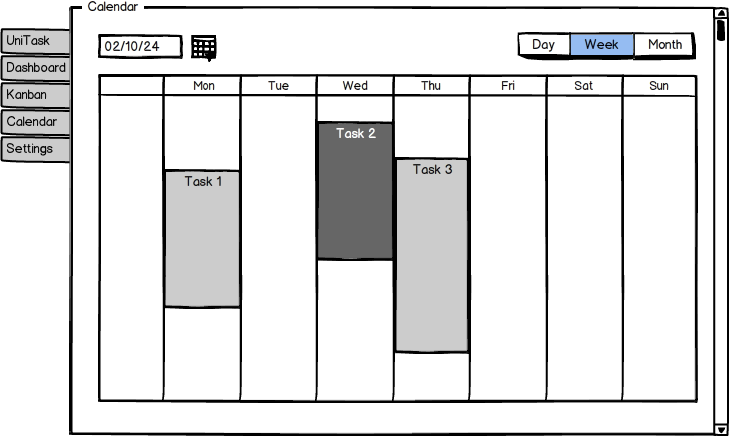
\includegraphics[width=0.65\textwidth]{mockups/Calendar}
%            \caption{\centering Mockup Calendar σελίδας}
%            \label{fig:unitaskMockupCalendar}
%        \end{figure}
%
%        \begin{figure}[h!] \noindent \centering
%            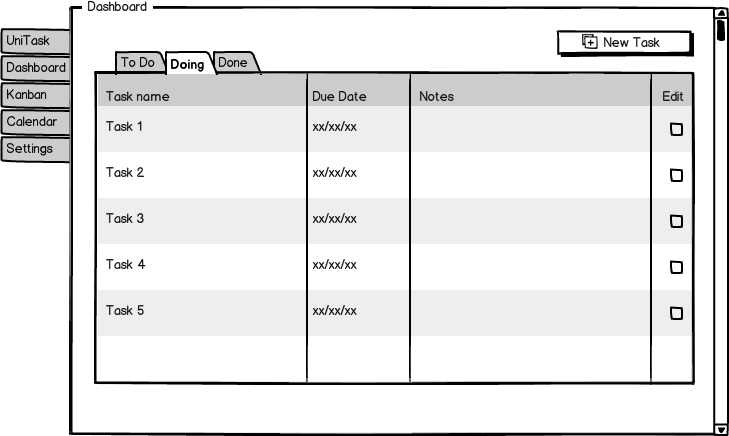
\includegraphics[width=0.65\textwidth]{mockups/Dashboard}
%            \caption{\centering Mockup Dashboard σελίδας}
%            \label{fig:unitaskMockupDashboard}
%        \end{figure}
%
%        \begin{figure}[h!] \noindent \centering
%            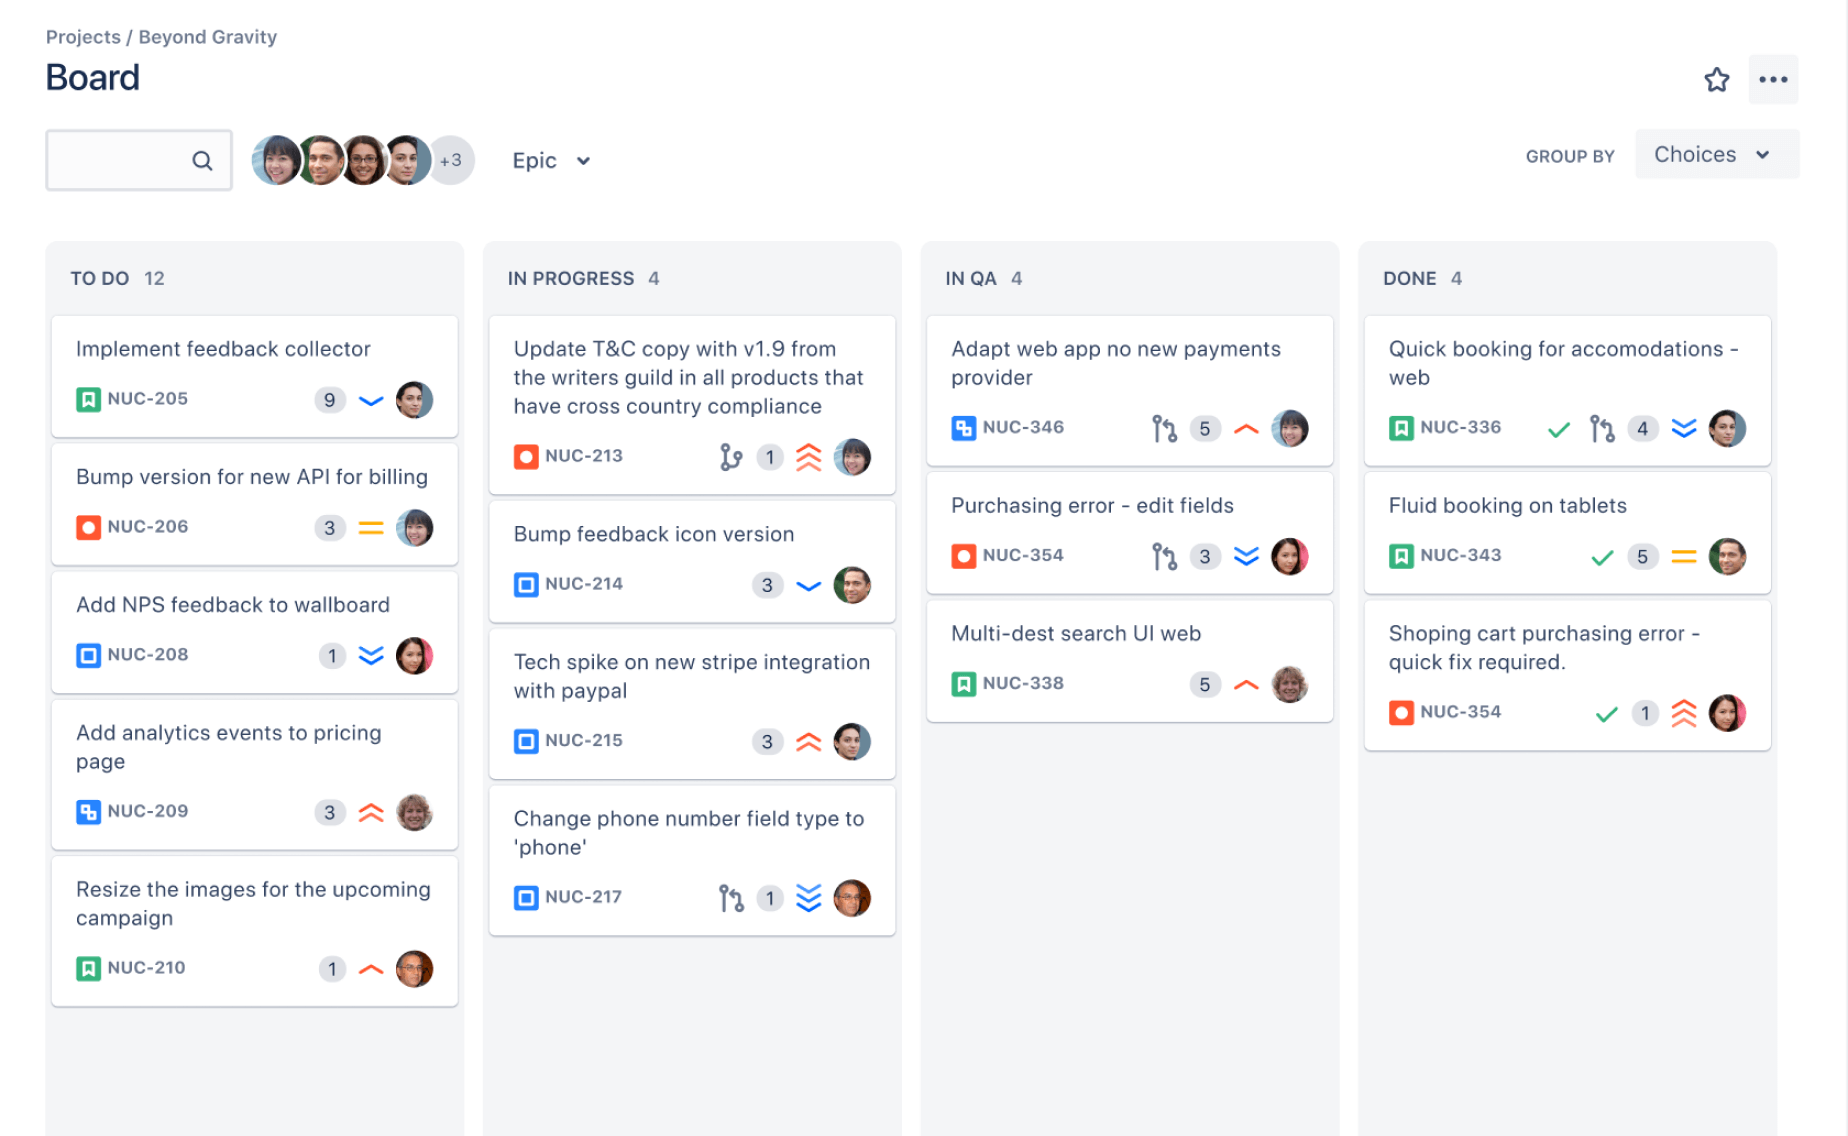
\includegraphics[width=0.65\textwidth]{mockups/Kanban}
%            \caption{\centering Mockup Kanban σελίδας}
%            \label{fig:unitaskMockupKanban}
%        \end{figure}
%
%    \pagebreak

%    \section{Η εφαρμογή}
%        Κατά την εκτέλεση της εφαρμογής, είτε τοπικά είτε μέσω της απομακρυσμένης πρόσβασης στο cloud, στη διεύθυνση \texttt{https://unitask-sandbox.mxapps.io/}, εμφανίζεται αρχικά η \textbf{σελίδα σύνδεσης}, όπως φαίνεται στο σχήμα \ref{fig:unitask_Login}. Στη συγκεκριμένη σελίδα, οι χρήστες καλούνται να εισάγουν τα στοιχεία σύνδεσής τους για να αποκτήσουν πρόσβαση στις λειτουργίες της εφαρμογής.
%
%        Ανάλογα με τα στοιχεία σύνδεσης που παρέχονται, το σύστημα διακρίνει δύο επίπεδα πρόσβασης: δικαιώματα διαχειριστή (Administrator) και δικαιώματα χρήστη (User), όπου εκπροσωπούν τους φοιτητές. Οι χρήστες με δικαιώματα Administrator έχουν πρόσβαση σε επιπλέον προηγμένες λειτουργίες διαχείρισης όπως η διαχείριση των χρηστών.
%
%       \begin{figure}[h!] \noindent \centering
%            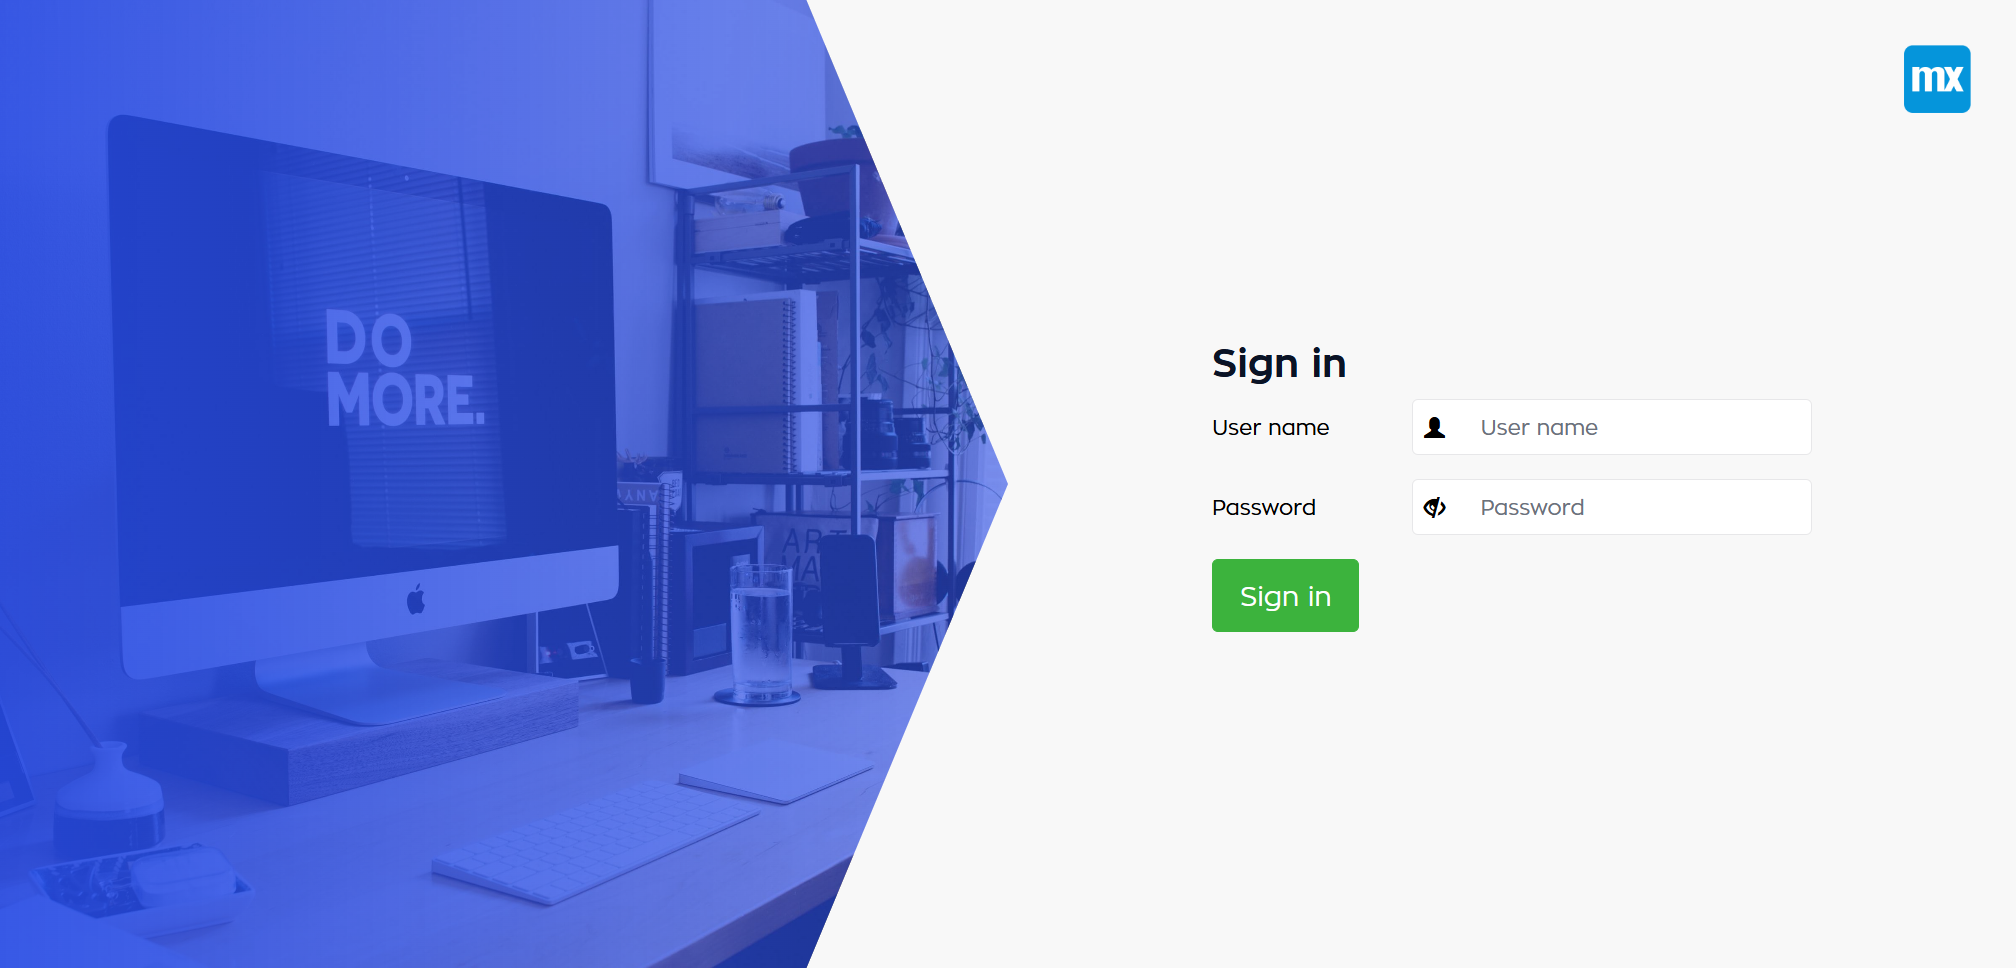
\includegraphics[width=\textwidth]{UniTask/Login}
%            \caption{\centering Σελίδα σύνδεσης}
%            \label{fig:unitask_Login}
%        \end{figure}
%
%        Αρχικά, πραγματοποιείται σύνδεση με τον λογαριασμό διαχειριστή (Administrator) προκειμένου να παρουσιαστούν οι λειτουργίες διαχείρισης χρηστών, συμπεριλαμβανομένης της δυνατότητας προσθήκης νέου χρήστη. Μετά την επιτυχή εισαγωγή των διαπιστευτηρίων του διαχειριστή, τα οποία έχουν οριστεί προκαταβολικά κατά την ανάπτυξη της εφαρμογής (βλ. ενότητα \ref{sec:unitask_mendix}), εμφανίζεται η \textbf{σελίδα διαχείρισης χρηστών}, όπως απεικονίζεται στο σχήμα \ref{fig:unitask_AccountOverview}. Η σελίδα αυτή παρέχει στους διαχειριστές μια ολοκληρωμένη επισκόπηση της λίστας χρηστών της εφαρμογής, καθώς και εργαλεία για τη διαχείρισή τους. Το layout της σελίδας αποτελείται από μια κάθετη μπάρα μενού η οποία περιλαμβάνει τις ίδιες δυνατότητες με τους απλούς χρήστες η οποίες θα αναλυθούν στη συνέχεια.
%
%       \begin{figure}[h!] \noindent \centering
%            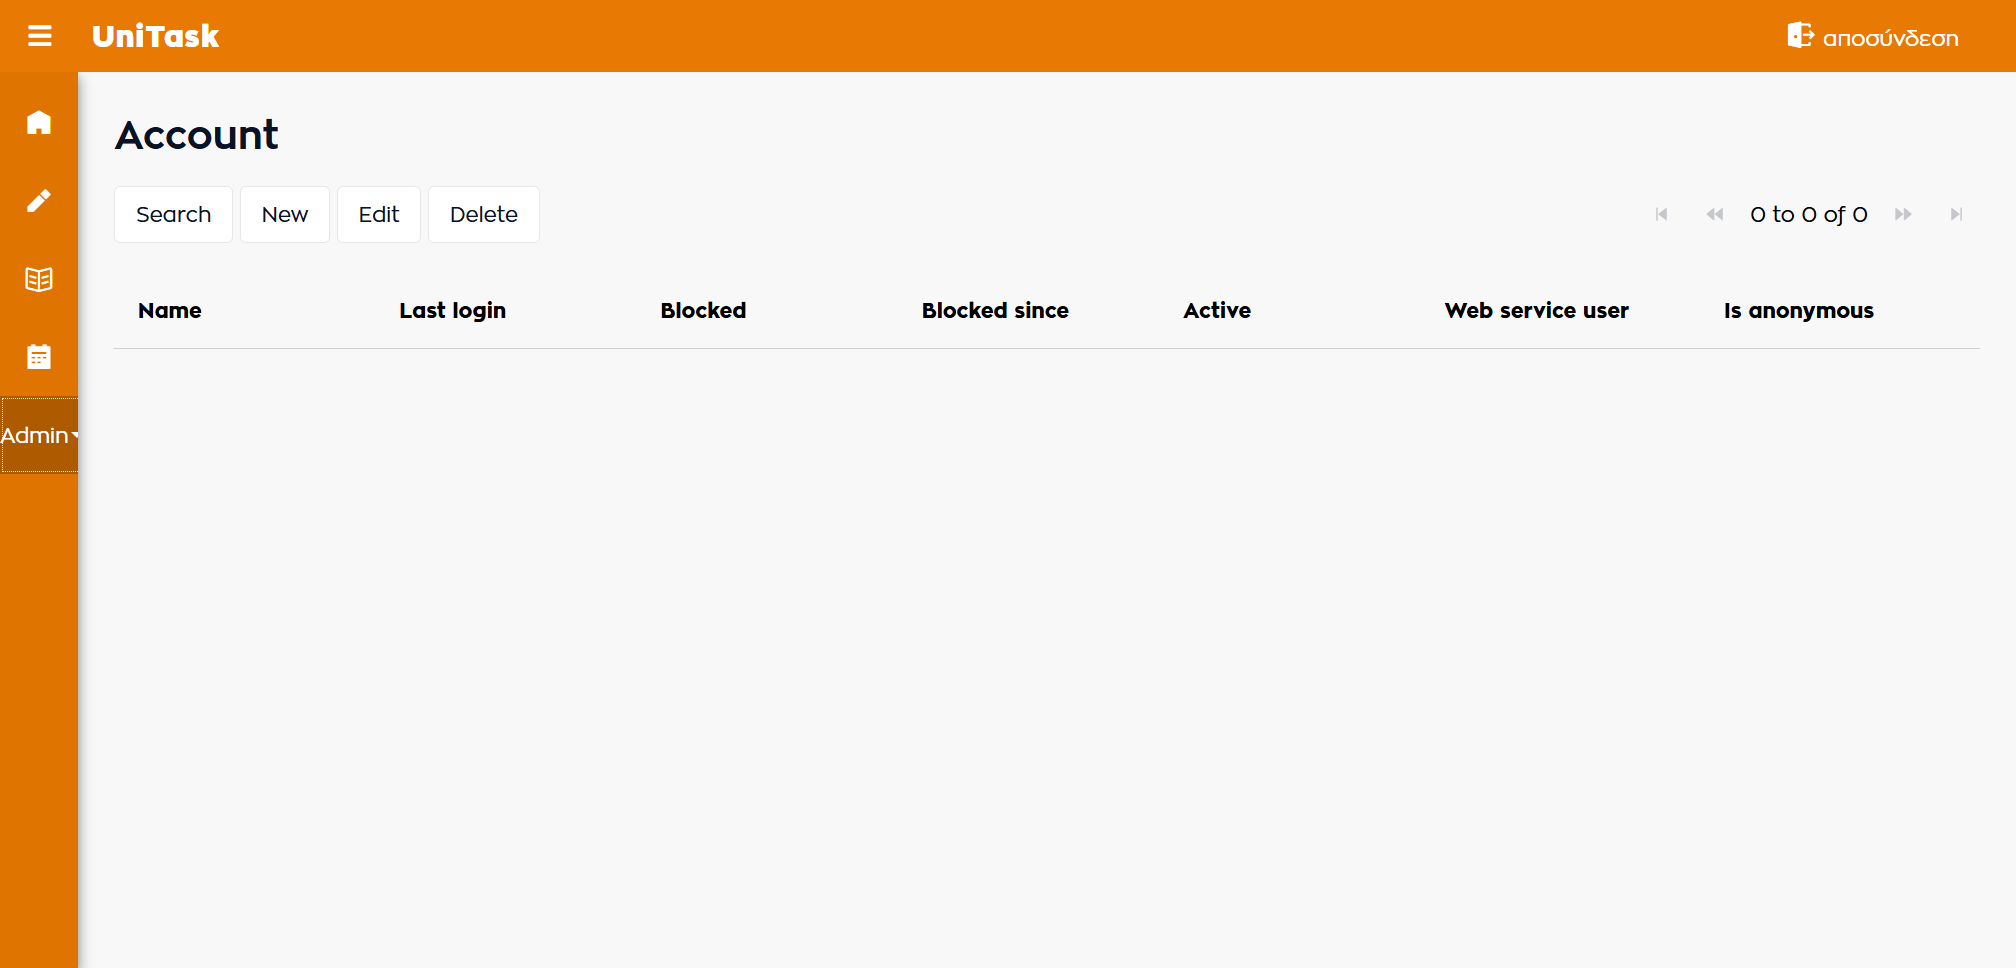
\includegraphics[trim={0 12cm 0 0}, clip, width=\textwidth]{UniTask/AccountOverview}
%            \caption{\centering Σελίδα διαχείρισης χρηστών}
%            \label{fig:unitask_AccountOverview}
%        \end{figure}
%
%        Πατώντας στο κουμπί {\Zona New}, εμφανίζεται η popout σελίδα του σχήματος \ref{fig:unitask_NewAccount} με μια \textbf{φόρμα για την προσθήκη νέου χρήστη}. Η φόρμα περιλαμβάνει πεδία για την εισαγωγή του ονόματος χρήστη ({\Zona Username}), του ρόλου του χρήστη ({\Zona User role}) όπου επιλέγεται αν πρόκειται για προσθήκη διαχειριστή ή χρήστη, του κωδικού πρόσβασης ({\Zona New password} και {\Zona Confirm password}). Λόγω του ότι ο χρήστης User έχει κληρονομήσει γνωρίσματα από την κλάση \texttt{System.User} του Mendix, έχουν προστεθεί πεδία όπως το {\Zona Blocked}, η οποία γίνεται αληθής μετά από κάποιες αποτυχημένες προσπάθειες σύνδεσης, το {\Zona Active} που γίνεται αληθές όταν ο χρήστης συνδεθεί, το {\Zona Time zone} όπου ορίζεται η ζώνη ώρας του χρήστη και το {\Zona Language} όπου ορίζεται η γλώσσα του χρήστη.
%
%        \begin{figure}[h!] \noindent \centering
%            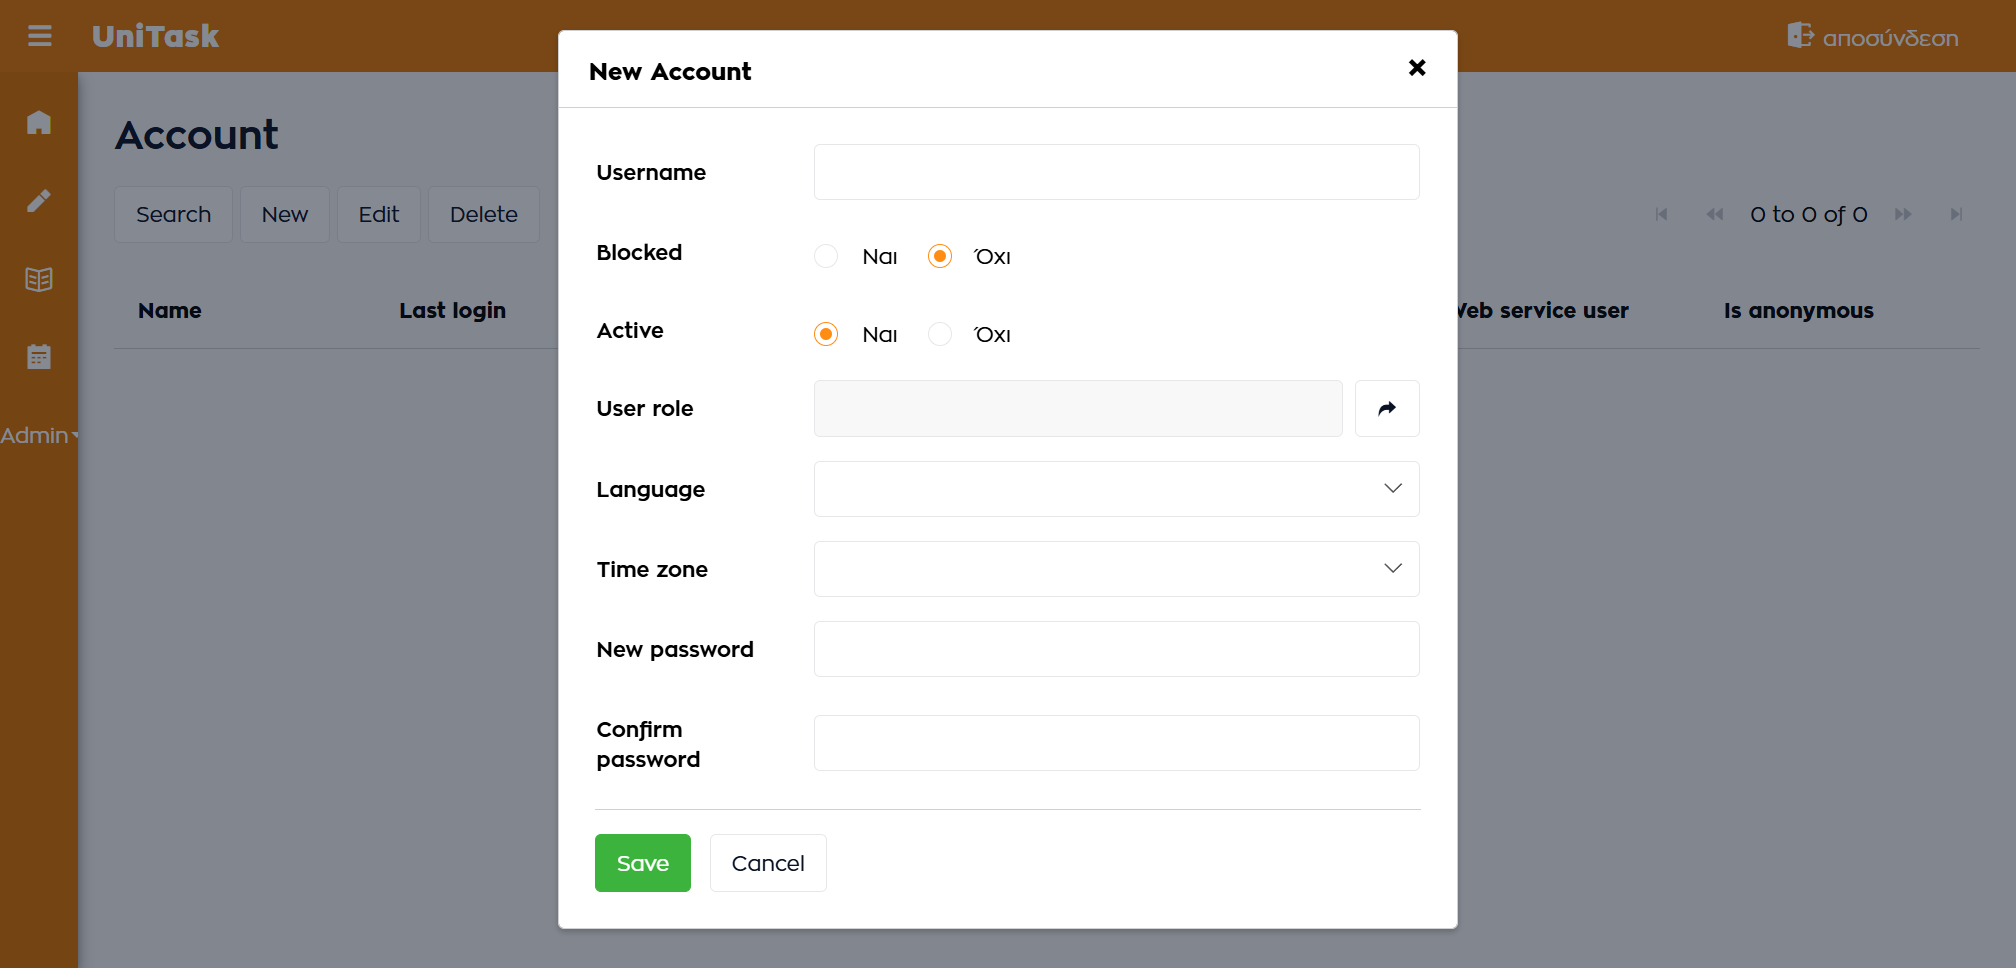
\includegraphics[width=\textwidth]{UniTask/NewAccount}
%            \caption{\centering Φόρμα προσθήκης νέου χρήστη}
%            \label{fig:unitask_NewAccount}
%        \end{figure}
%
%        Δημιουργούμε έναν χρήστη με όνομα \texttt{Foithths}, ο οποίος εμφανίζεται στη λίστα των χρηστών (σχήμα \ref{fig:unitask_AccountOverview_WithStudent}. Πατώντας στο όνομά του, εμφανίζεται η σελίδα επεξεργασίας του χρήστη, όπως φαίνεται στο σχήμα \ref{fig:unitask_EditAccount}. Στη λίστα των χρηστών υπάρχει η δυνατότητα αναζήτησης χρηστών βάσει όλων των στοιχείων τους (σχήμα \ref{fig:unitask_SearchAccounts}), όπως επίσης και η δυνατότητα διαγραφής τους.
%
%        \begin{figure}[h!] \noindent \centering
%            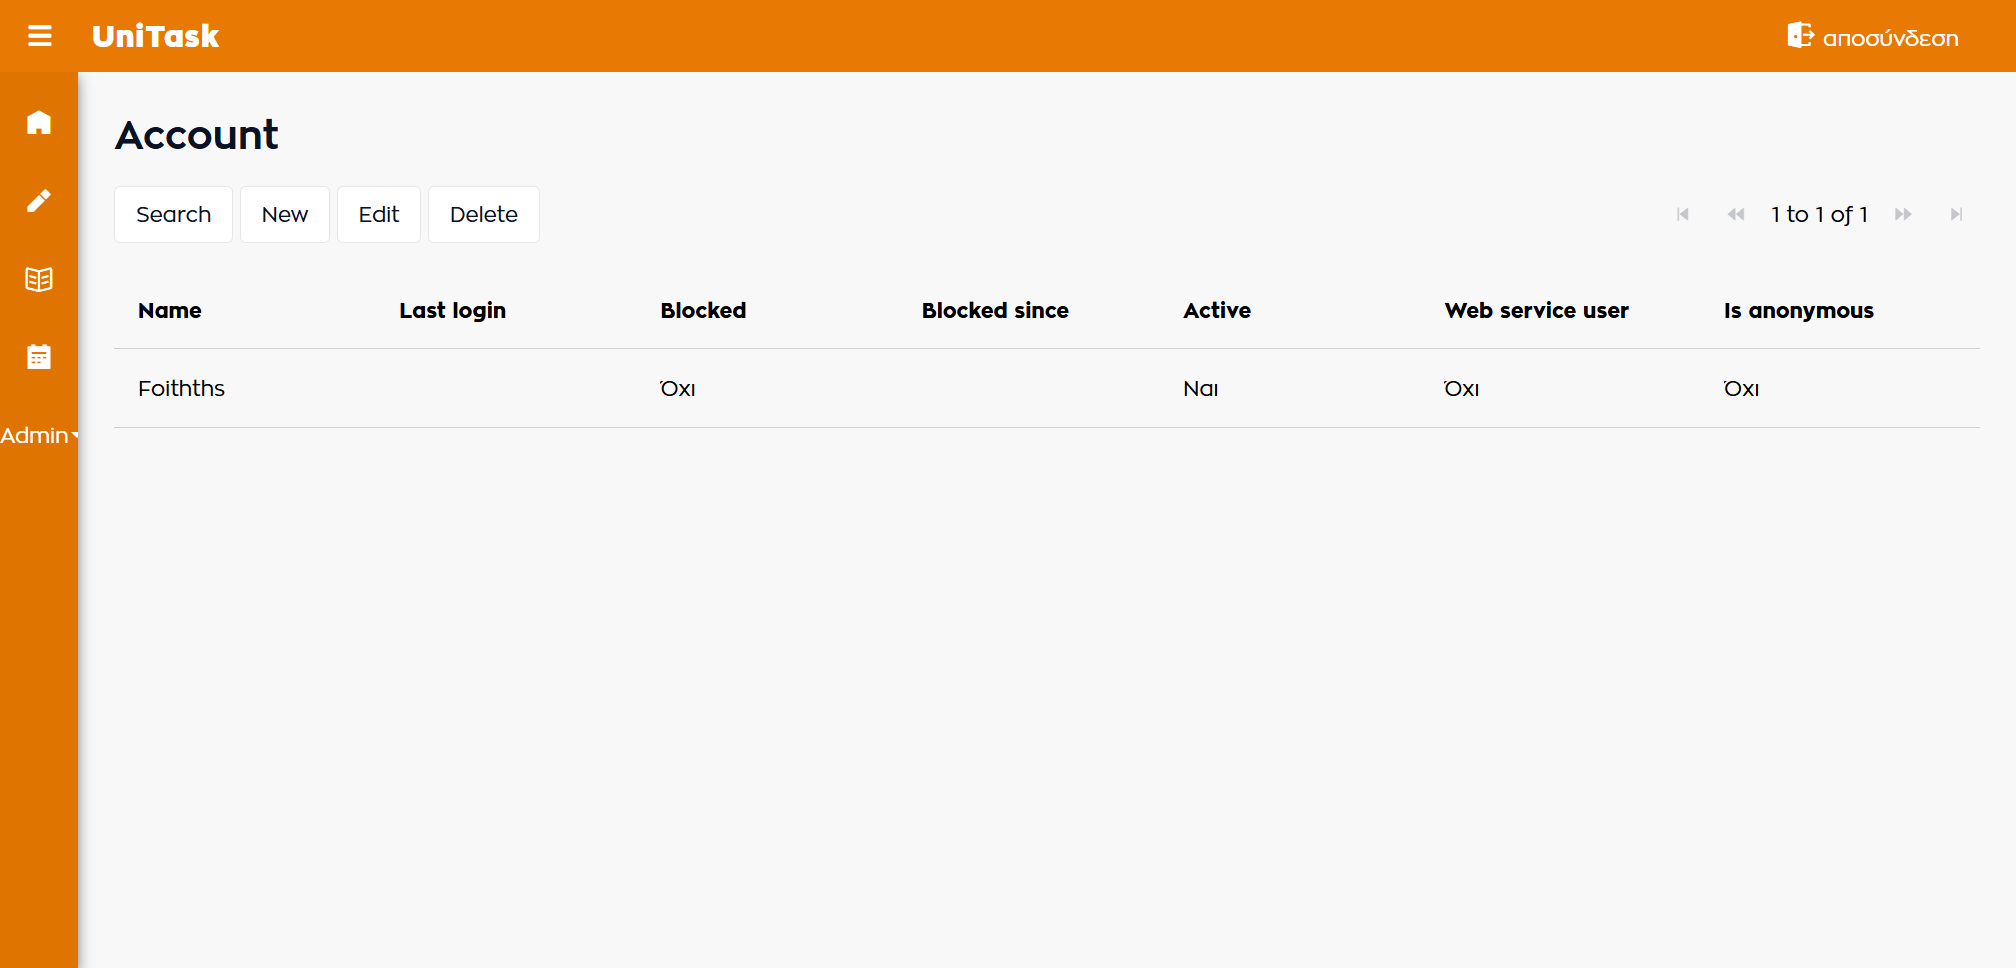
\includegraphics[trim={0 17cm 0 0}, clip, width=\textwidth]{UniTask/AccountOverview_WithStudent}
%            \caption{\centering Λίστα χρηστών με τον χρήστη \texttt{Foithths}}
%            \label{fig:unitask_AccountOverview_WithStudent}
%        \end{figure}
%
%        \begin{figure}[h!] \noindent \centering
%            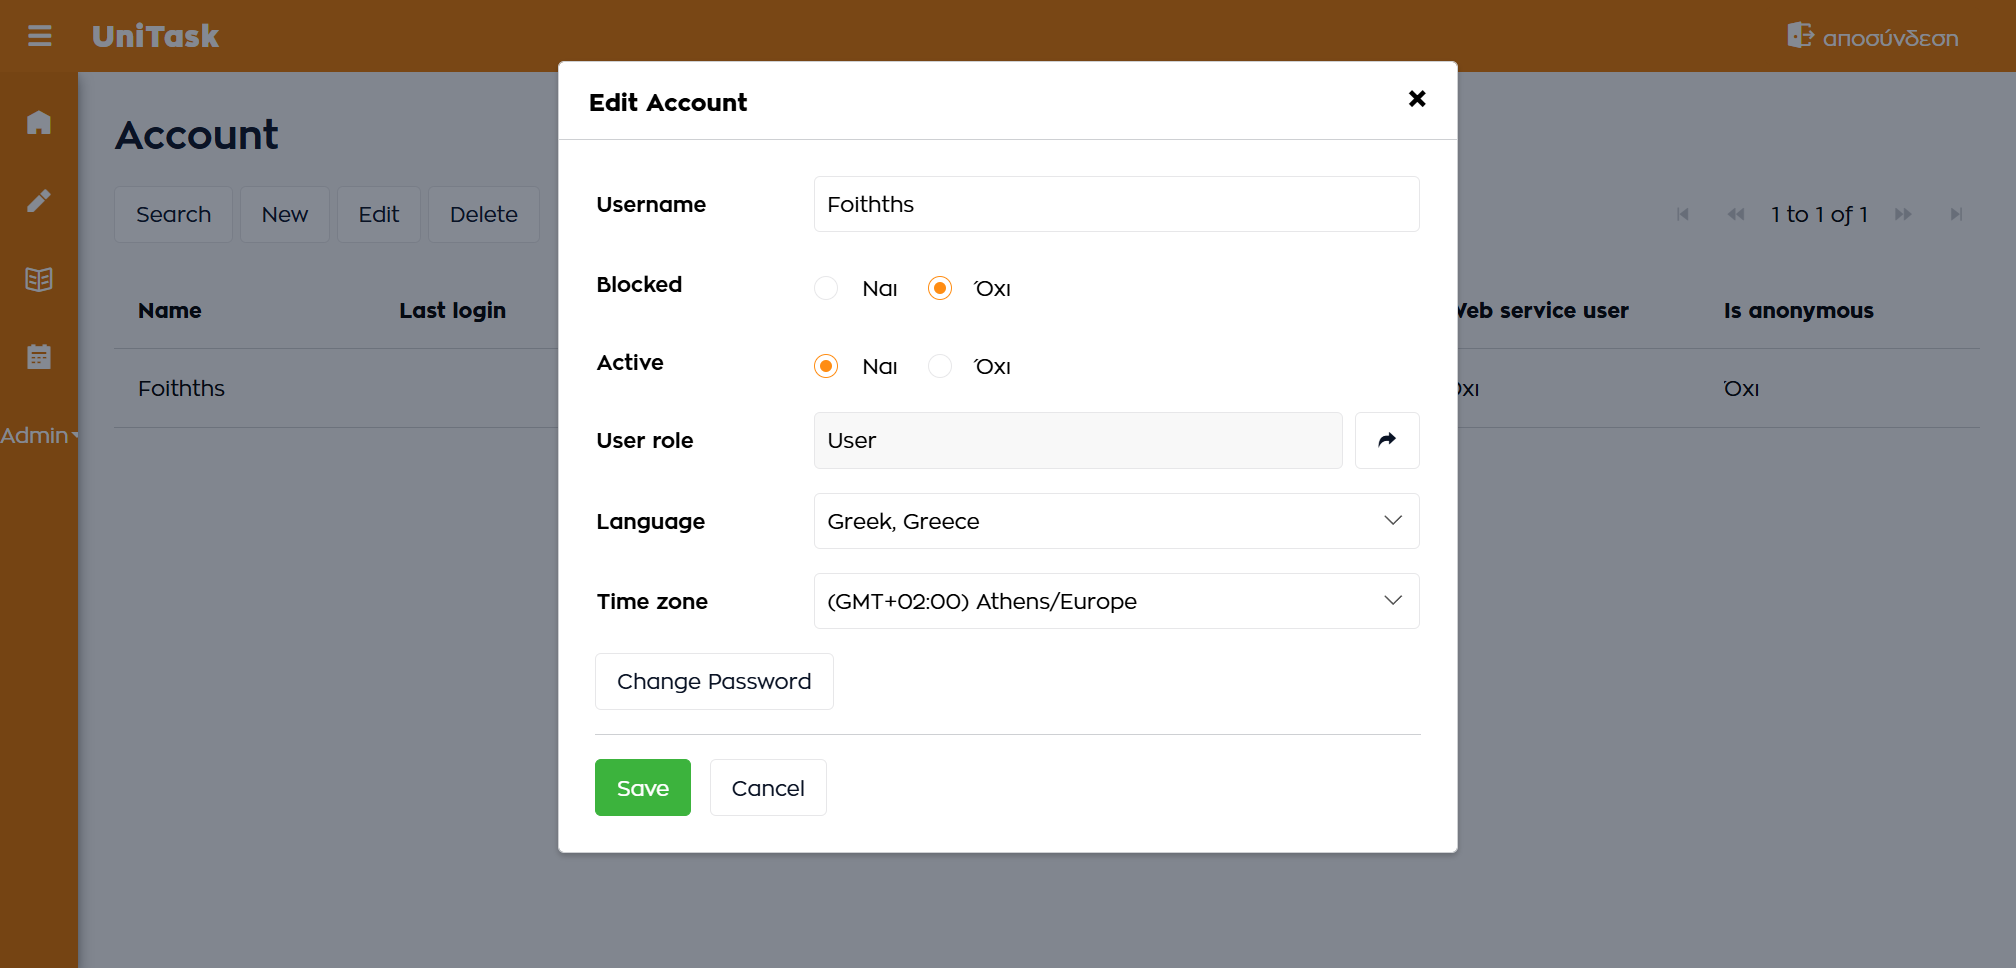
\includegraphics[trim={0 3cm 0 0}, clip, width=\textwidth]{UniTask/EditAccount}
%            \caption{\centering Επεξεργασία στοιχείων χρήστη}
%            \label{fig:unitask_EditAccount}
%        \end{figure}
%
%        \begin{figure}[h!] \noindent \centering
%            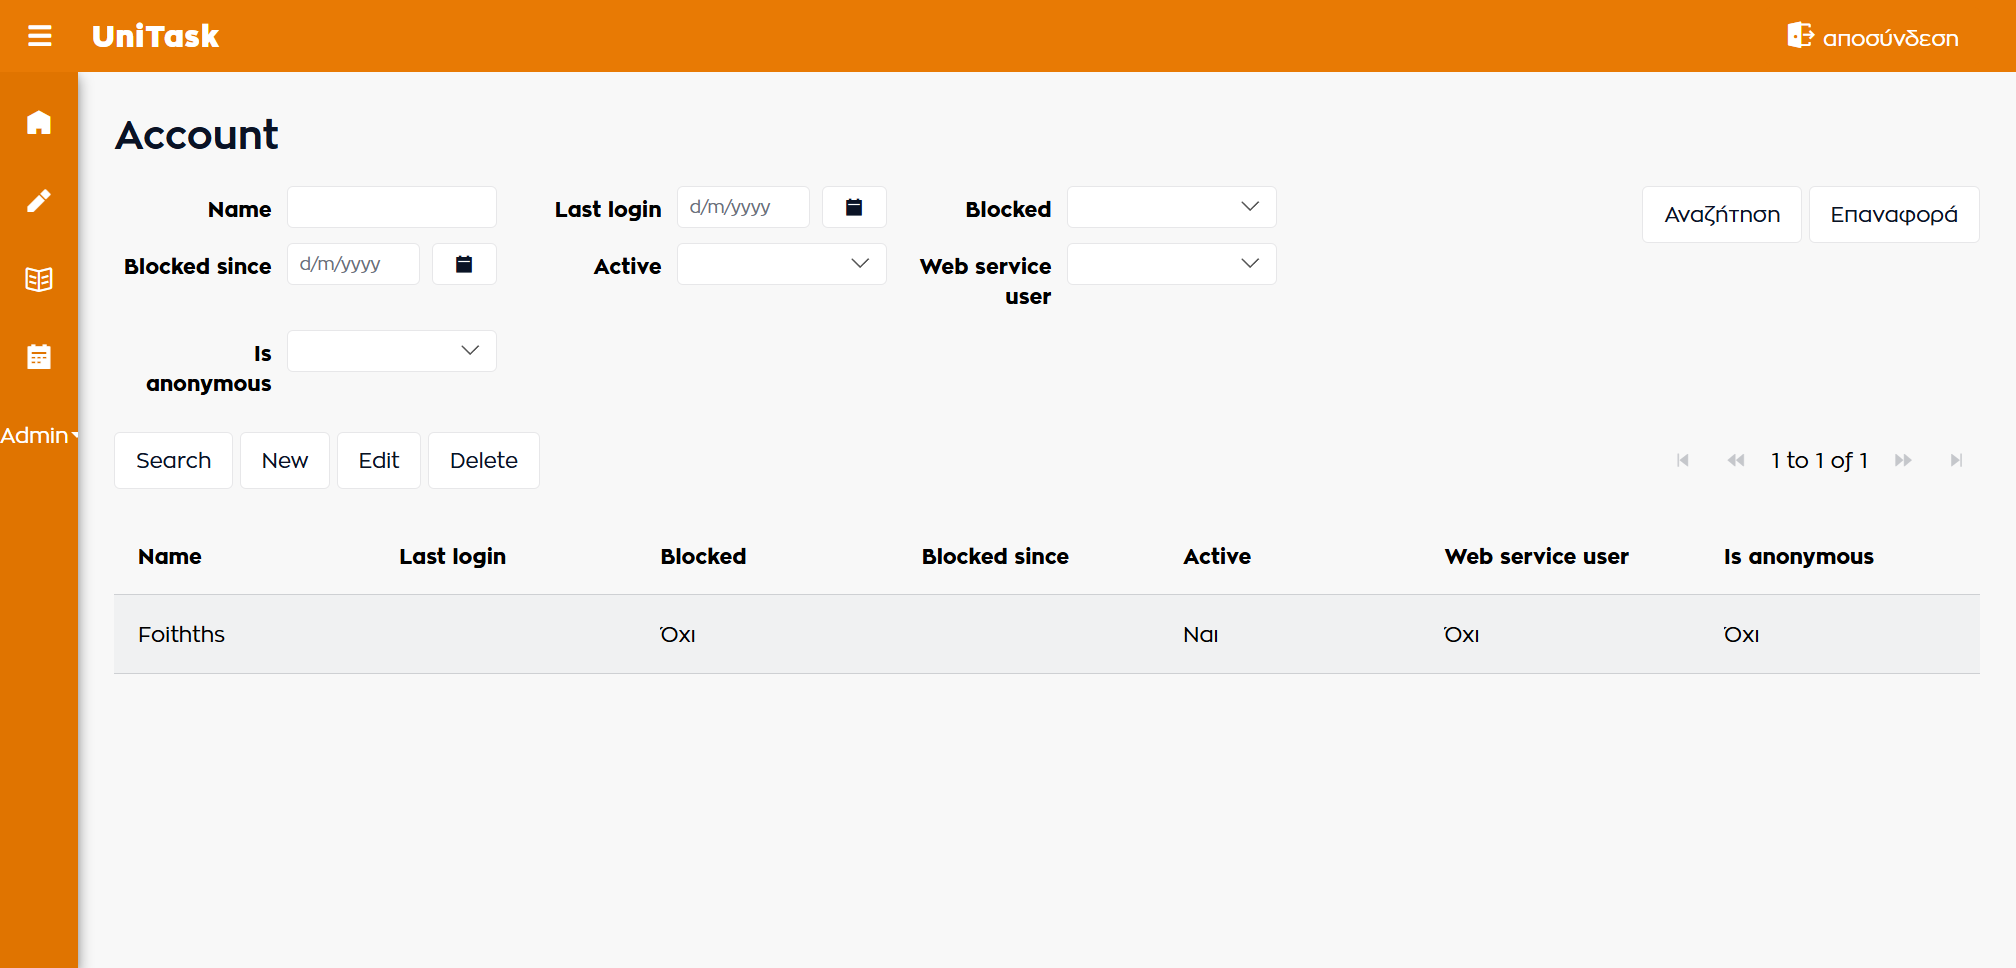
\includegraphics[trim={0 7cm 0 0}, clip, width=\textwidth]{UniTask/SearchAccounts}
%            \caption{\centering Αναζήτηση χρήστη}
%            \label{fig:unitask_SearchAccounts}
%        \end{figure}
%
%        Αφού αποσυνδεθούμε και συνδεθούμε ως \texttt{Foithths}, μας υποδέχεται η \textbf{αρχική σελίδα} της εφαρμογής (σχήμα \ref{fig:unitask_Home}). Η σελίδα περιλαμβάνει ένα κεντρικό call to action κουμπί ({\Zona όλες οι εργασίες}) το οποίο οδηγεί στο {\Zona dashboard}.
%
%        \begin{figure}[h!] \noindent \centering
%            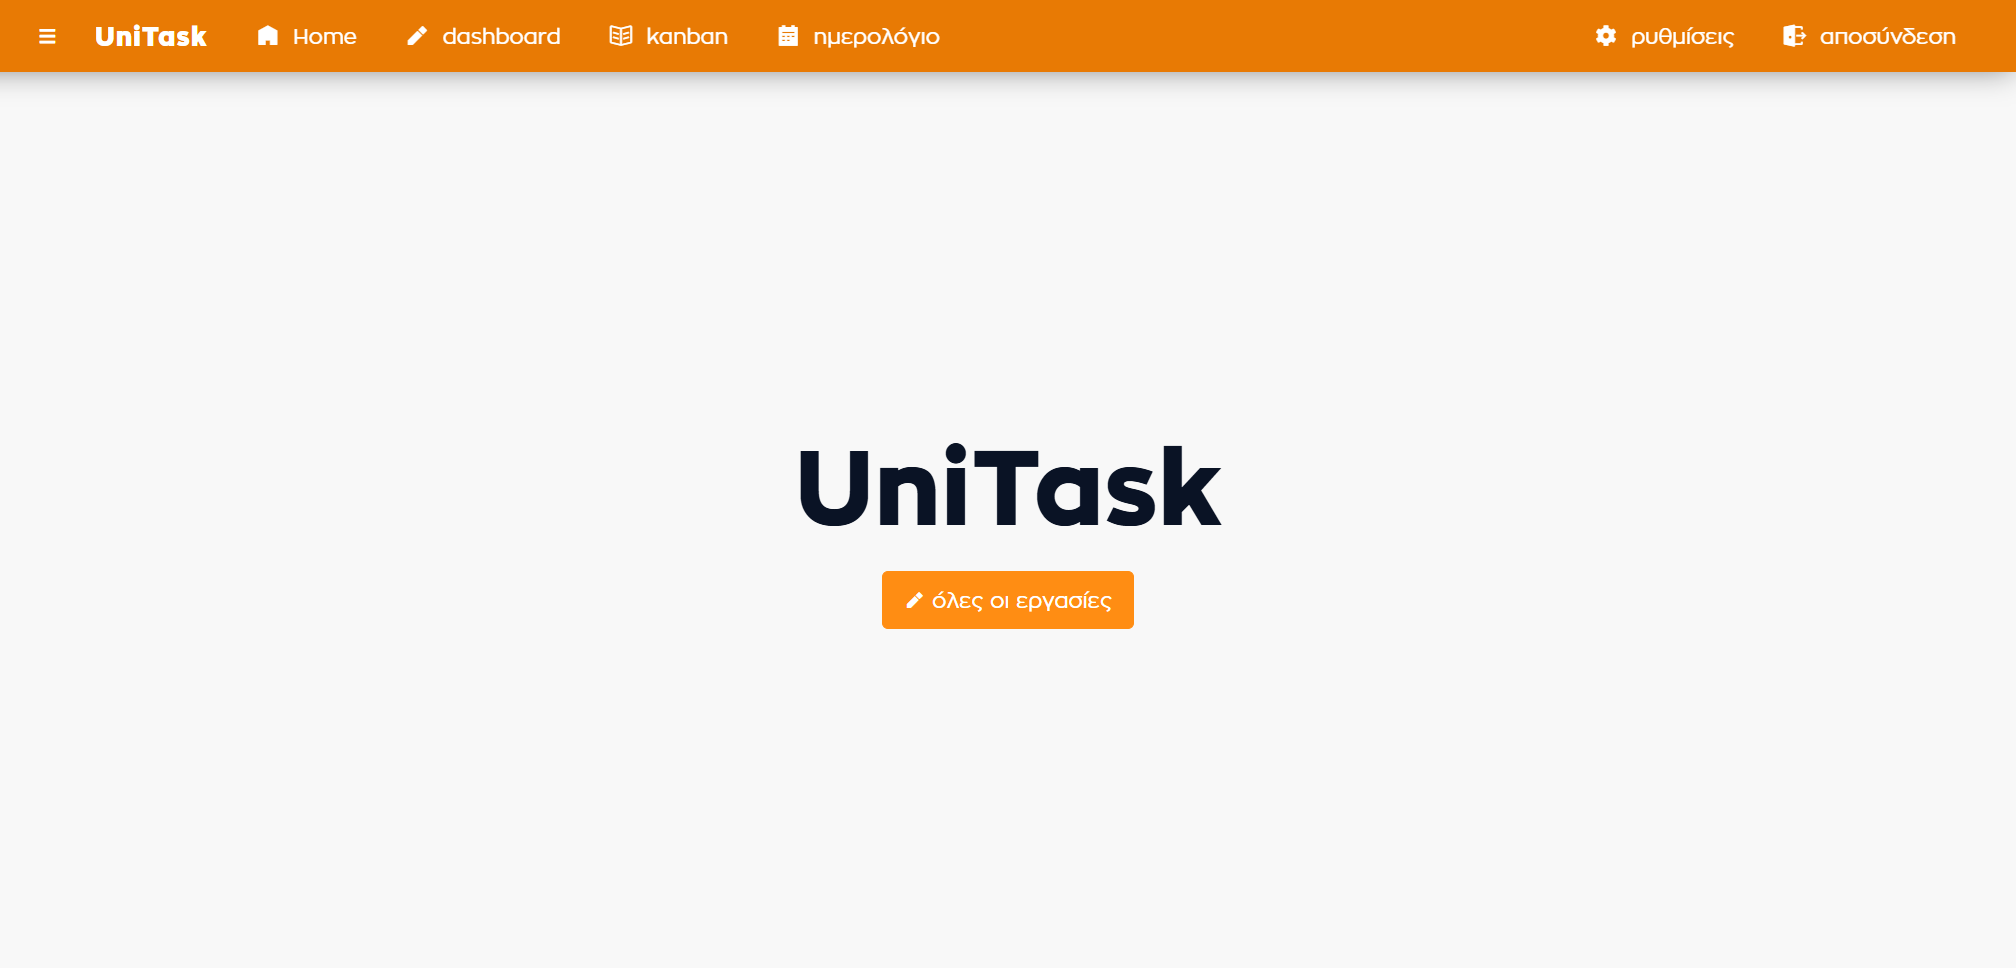
\includegraphics[width=\textwidth]{UniTask/Home}
%            \caption{\centering Αρχική σελίδα εφαρμογής}
%            \label{fig:unitask_Home}
%        \end{figure}
%
%        \begin{figure}[h!] \noindent \centering
%            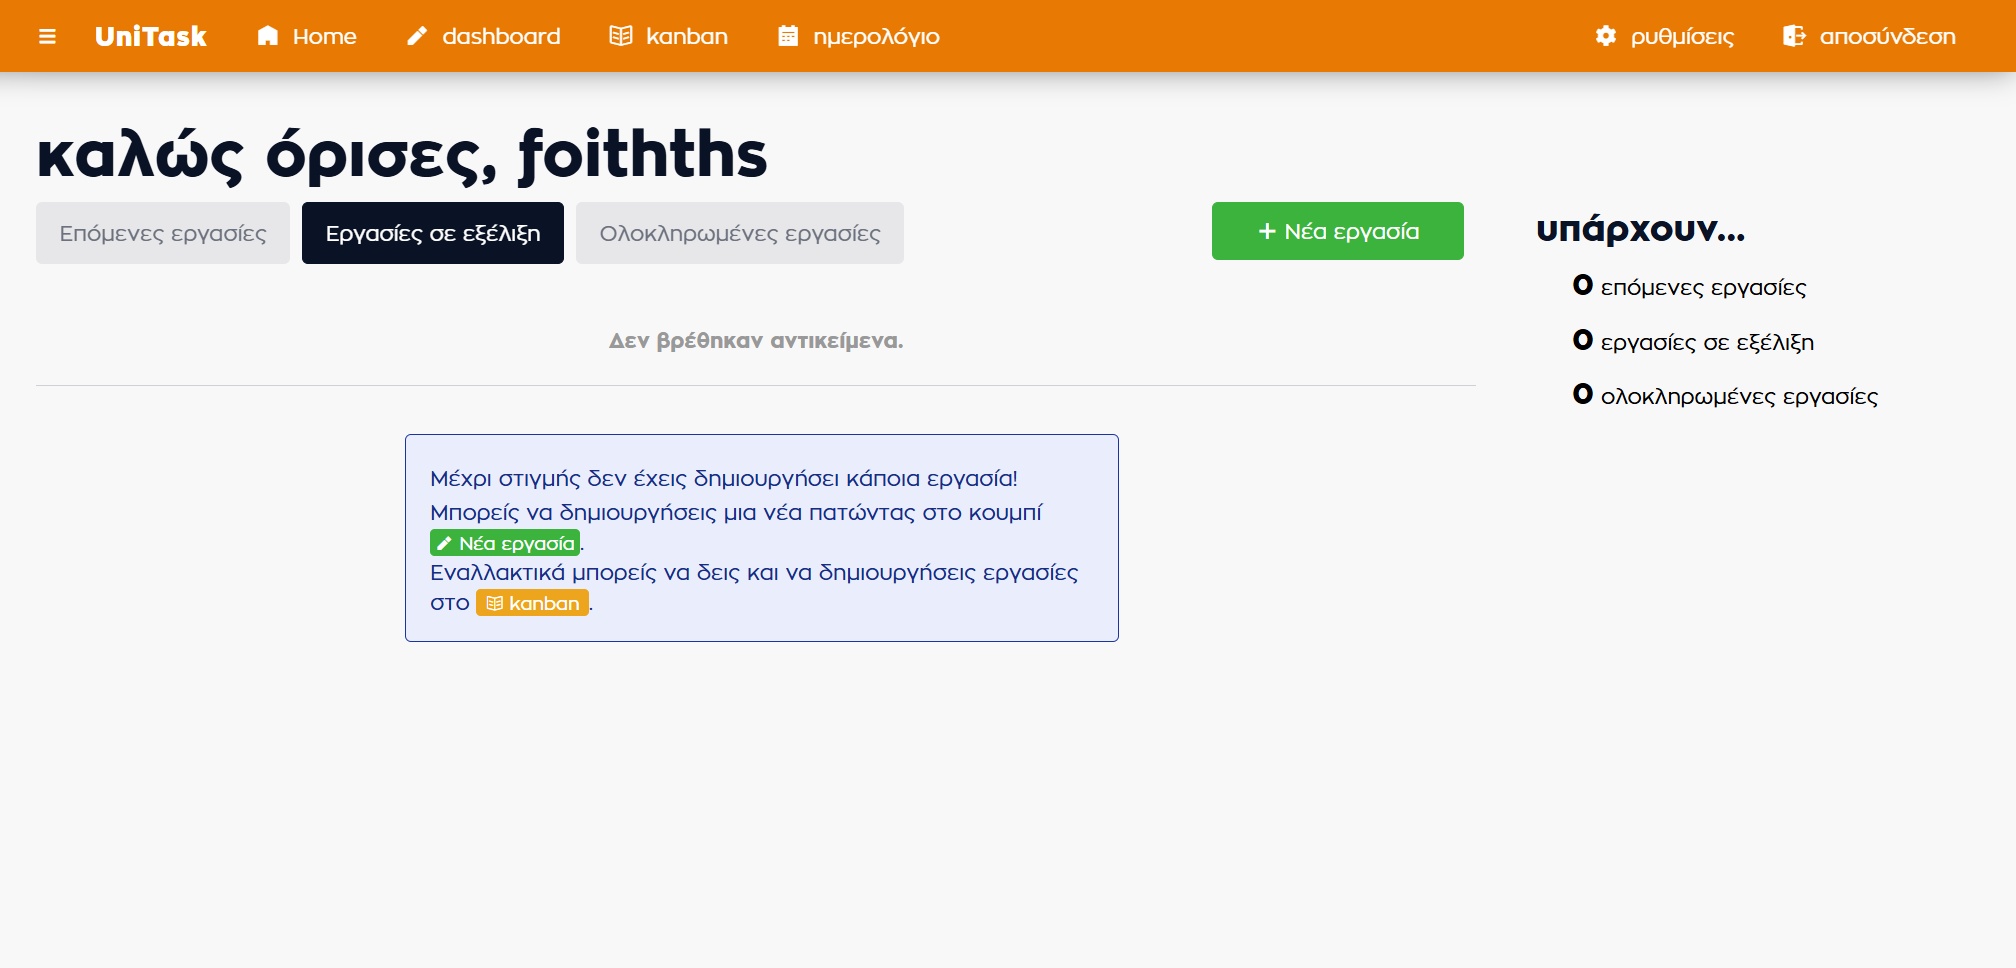
\includegraphics[width=\textwidth]{UniTask/TaskDashboard}
%            \caption{\centering Dashboard εργασιών}
%            \label{fig:unitask_TaskDashboard}
%        \end{figure}
%
%        Στο σχήμα \ref{fig:unitask_TaskDashboard} εμφανίζεται η σελίδα {\ZonaSB dashboard}. Πρόκειται για την κεντρική σελίδα προβολής, δημιουργίας και επεξεργασίας των εργασιών του χρήστη. Περιλαμβάνονται τρεις καρτέλες ({\Zona Επόμενες εργασίες}, {\Zona Εργασίες σε εξέλιξη}, {\Zona Ολοκληρωμένες εργασίες}). Οι επόμενες εργασίες αφορούν εργασίες που έχουν σκοπό να πραγματοποιηθούν στο άμεσο μέλλον αλλά όχι τη δεδομένη χρονική στιγμή, οι εργασίες σε εξέλιξη αφορούν εργασίες που βρίσκονται σε εξέλιξη και οι ολοκληρωμένες εργασίες αφορούν εργασίες που έχουν ολοκληρωθεί.
%
%        Στη σελίδα επίσης περιλαμβάνεται ένα επεξηγηματικό παράθυρο που εμφανίζεται μόνο όταν ο χρήστης δεν έχει δημιουργήσει κάποια εργασία και του εξηγεί το τρόπο λειτουργίας της εφαρμογής. Στο {\Zona dashboard} επίσης περιλαμβάνονται μετρητές για το σύνολο των εργασιών που υπάρχουν ανά κατηγορία, όπως επίσης και ένα κεντρικό κουμπί δημιουργίας εργασιών ({\Zona Νέα εργασία}).
%
%        \begin{figure}[h!] \noindent \centering
%            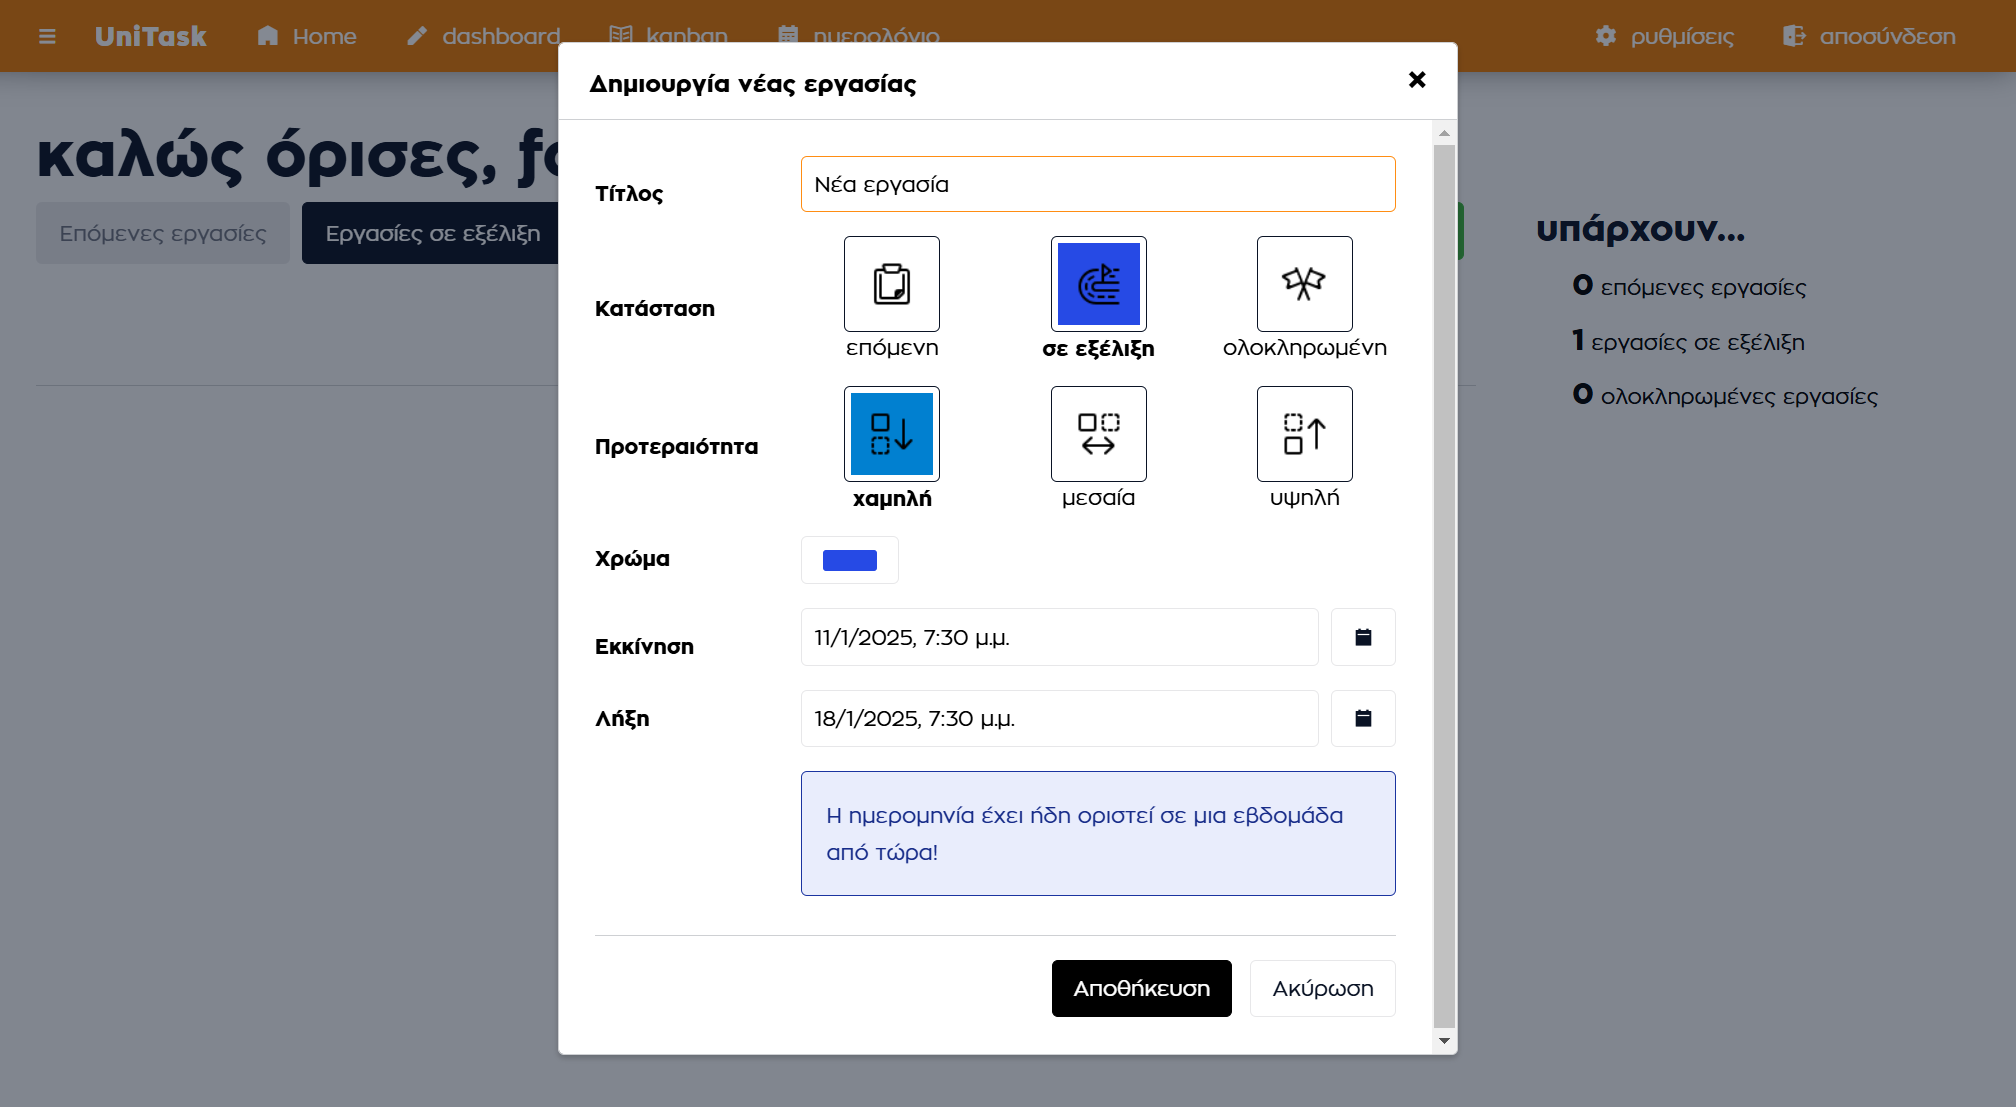
\includegraphics[width=\textwidth]{UniTask/NewTask_Default}
%            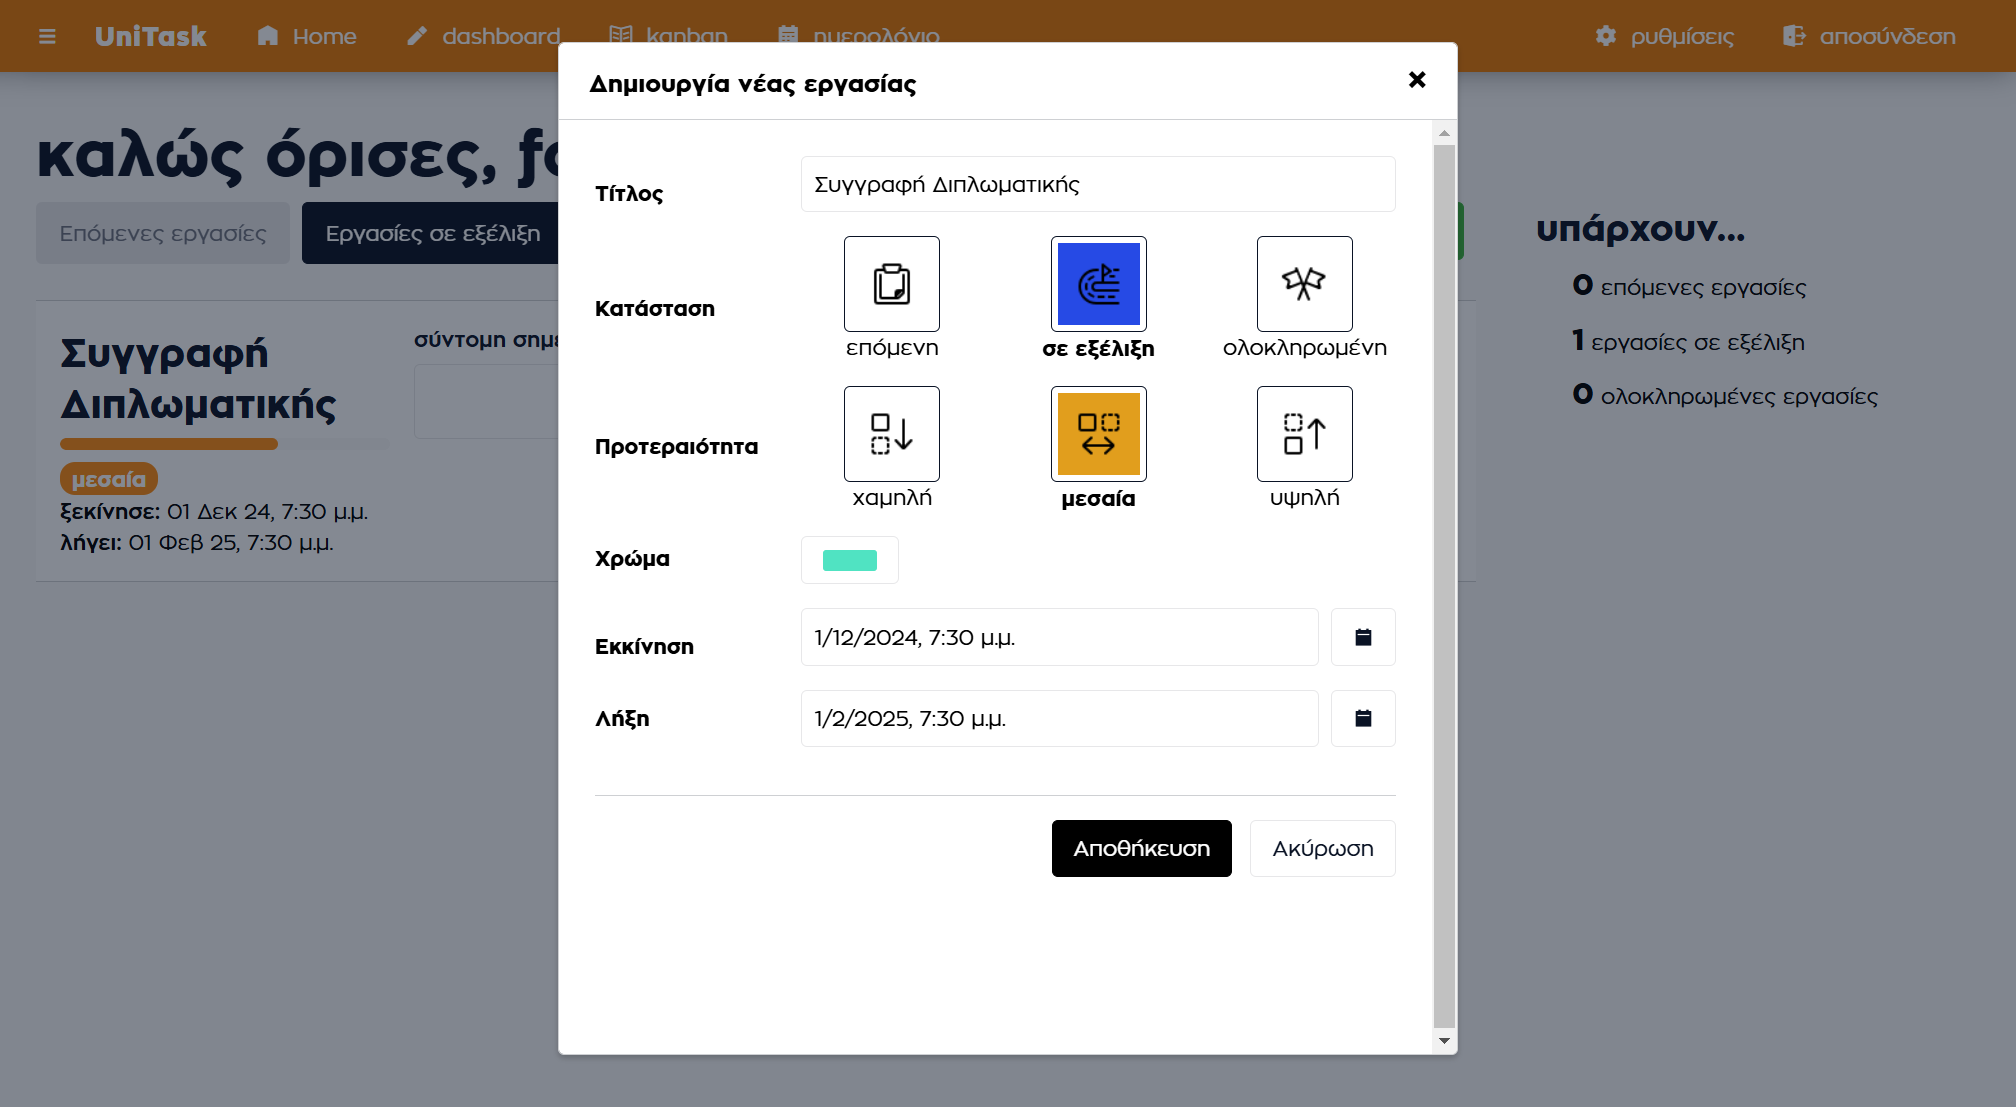
\includegraphics[width=\textwidth]{UniTask/NewTask_Finished}
%            \caption{\centering Δημιουργία νέας εργασίας}
%            \label{fig:unitask_NewTask}
%        \end{figure}
%
%        Πατώντας το, εμφανίζεται ένα popout παράθυρο (σχήμα \ref{fig:unitask_NewTask}.1) με μια φόρμα για τη δημιουργία μιας νέας εργασίας. Η φόρμα αυτή περιλαμβάνει πεδία για την εισαγωγή του τίτλου της εργασίας ({\Zona Τίτλος}), της ημερομηνίας έναρξης ({\Zona Εκκίνηση}) και λήξης ({\Zona Λήξη}), της κατάστασης της εργασίας ({\Zona Κατάσταση}), της προτεραιότητας της εργασίας ({\Zona Προτεραιότητα}) όπως επίσης και του χρώματος της εργασίας ({\Zona Χρώμα}), όπως θα αποτυπωθεί μετέπειτα στο ημερολόγιο. Στο popout παράθυρο ορίζεται προεπιλεγμένα ως ημερομηνία λήξης της εργασίας μια εβδομάδα μετέπειτα από την ημερομηνία δημιουργίας της, ενώ η κατάσταση της εργασίας έχει προκαθοριστεί (γίνεται να τροποποιηθεί φυσικά) ανάλογα με το ποια καρτέλα ήταν ανοιχτή στο dashboard. Αφού επεξεργαστούμε το παράθυρο όπως επιθυμούμε (σχήμα \ref{fig:unitask_NewTask}.2), πατάμε αποθήκευση για την αποθήκευση της εργασίας.
%
%        Να σημειωθεί πως οι επιλογές που αφορούν την κατάσταση και την προτεραιότητα της εργασίας είναι χρωματικά ταξινομημένες (color-coded) με το δικό τους γραφικό σύμβολο, όπως φαίνεται στο σχήμα \ref{fig:unitask_NewTask_AllOptions}, με σκοπό να διευκολύνει τον χρήστη για την άμεση αναγνώριση τους.
%
%        \begin{figure}[h!] \noindent \centering
%            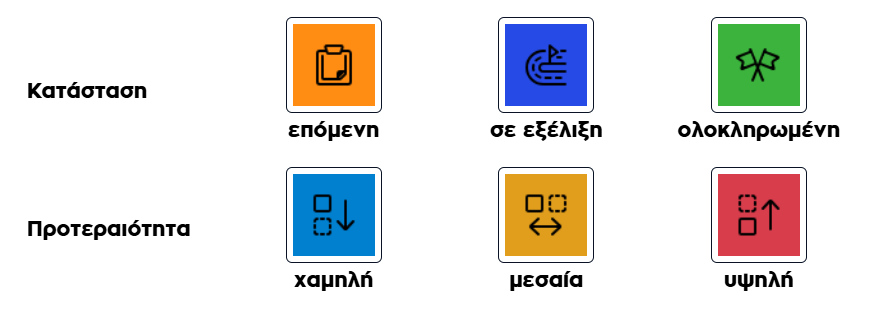
\includegraphics[width=0.7\textwidth]{UniTask/NewTask_AllOptions}
%            \caption{\centering Επιλογές κατάστασης και προτεραιότητας εργασίας}
%            \label{fig:unitask_NewTask_AllOptions}
%        \end{figure}
%
%        \begin{figure}[h!] \noindent \centering
%            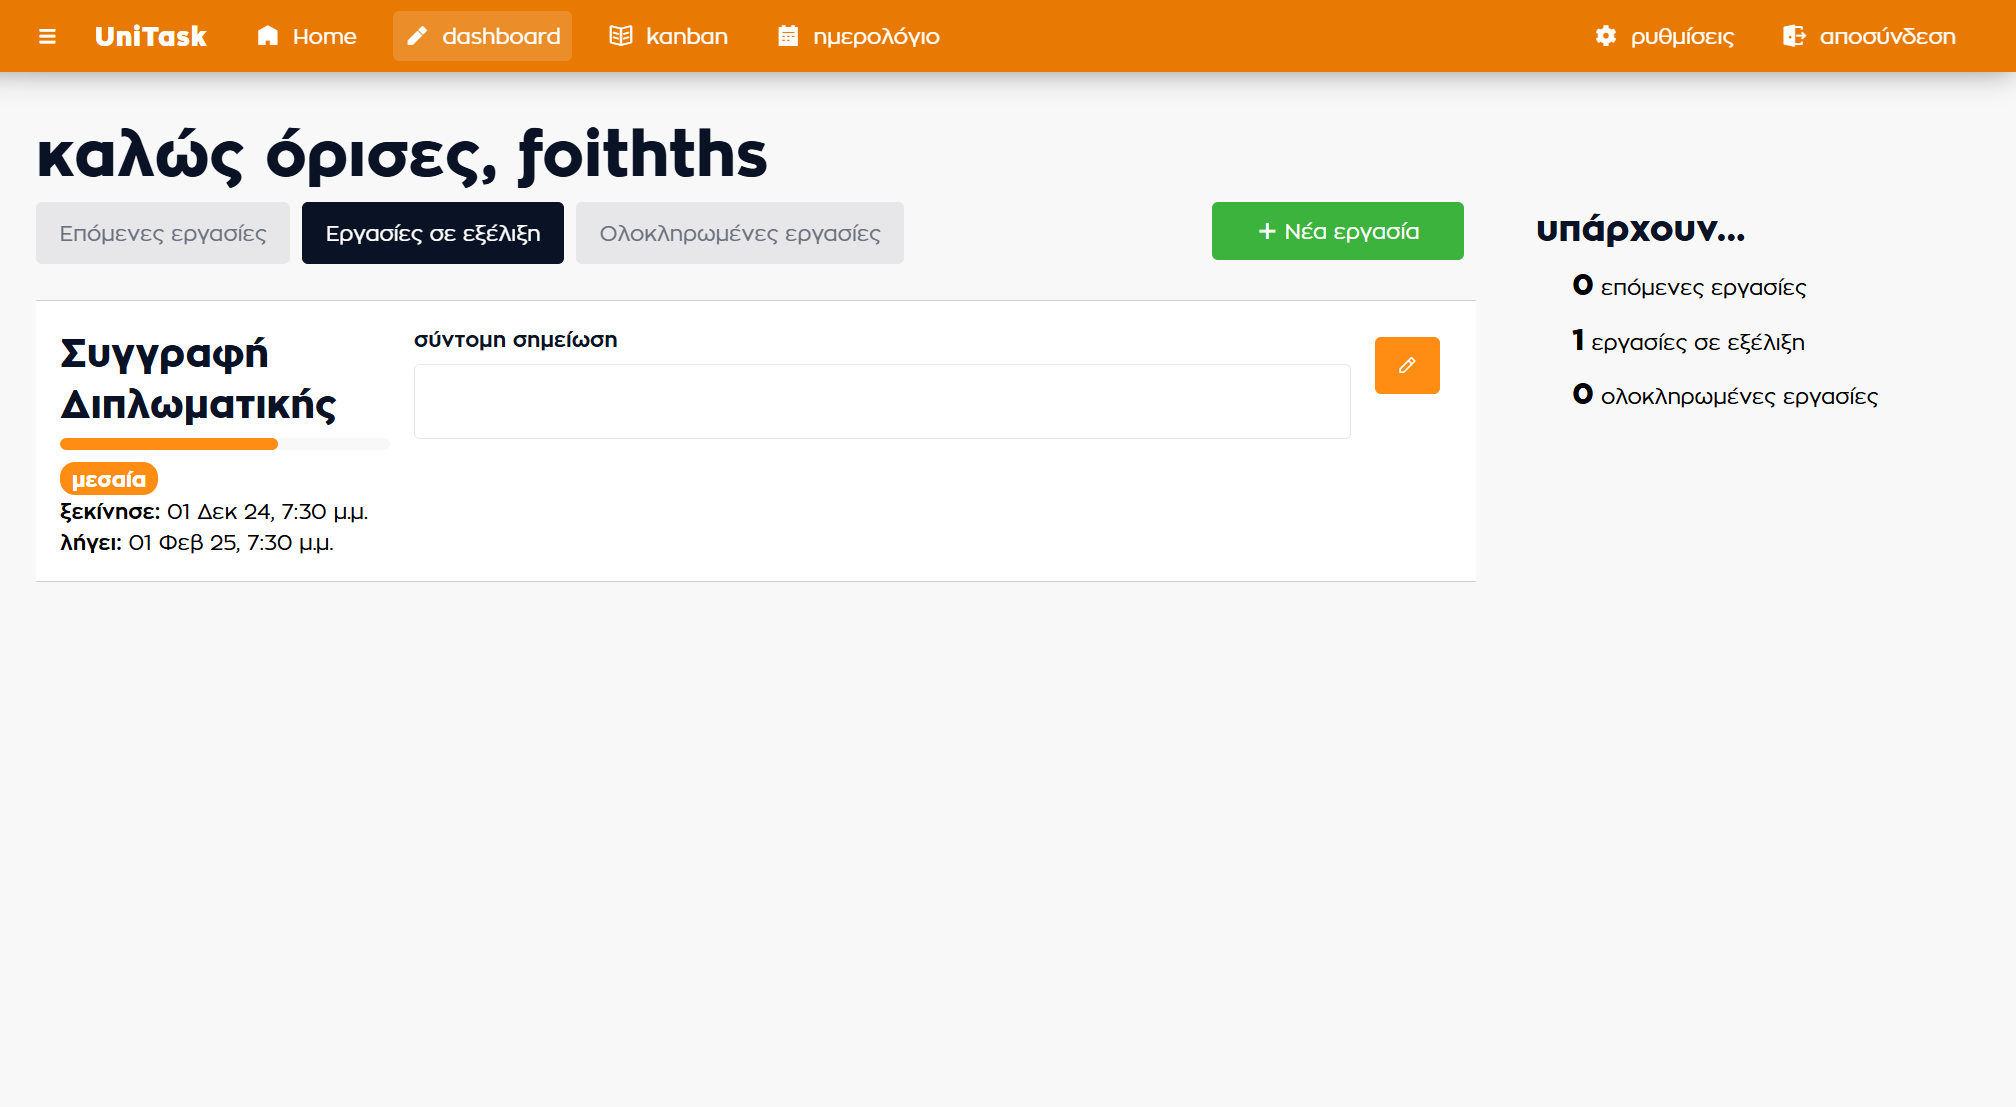
\includegraphics[trim={0 10cm 0 0}, clip, width=\textwidth]{UniTask/TaskDashboard_WithTask}
%            \caption{\centering Dashboard με δημιουργημένη εργασία}
%            \label{fig:unitask_TaskDashboard_WithTask}
%        \end{figure}
%
%        Στη σελίδα πλέον είναι δημιουργημένη η κάρτα με την πρώτη μας εργασία (σχήμα \ref{fig:unitask_TaskDashboard_WithTask}). Στο πλαίσιο {\Zona σύντομη σημείωση} μπορούμε να προσθέσουμε μια σύντομη περιγραφή της εργασίας, στα αριστερά εμφανίζεται ο τίτλος της εργασίας, μια μπάρα προόδου (progress bar) η οποία δυναμικά αυξάνεται όσο πλησιάζουμε στη λήξη της εργασίας, όπως επίσης η προτεραιότητα της εργασίας και οι ημερομηνίες και ώρες εκκίνησης και λήξης της εργασίας, ενώ στο δεξί μέρος της κάρτας εμφανίζονται το εικονίδιο για την επεξεργασία της εργασίας.
%
%        Ο τρόπος εμφάνισης των εργασιών στο dashboard λαμβάνει υπόψη του την προτεραιότητα τους και τον χρόνο λήξης τους. Έτσι μια εργασία με υψηλή προτεραιότητα θα εμφανίζεται ψηλότερα από μια εργασία με χαμηλή προτεραιότητα που δε λήγει σύντομα.
%
%        \begin{figure}[h!] \noindent \centering
%            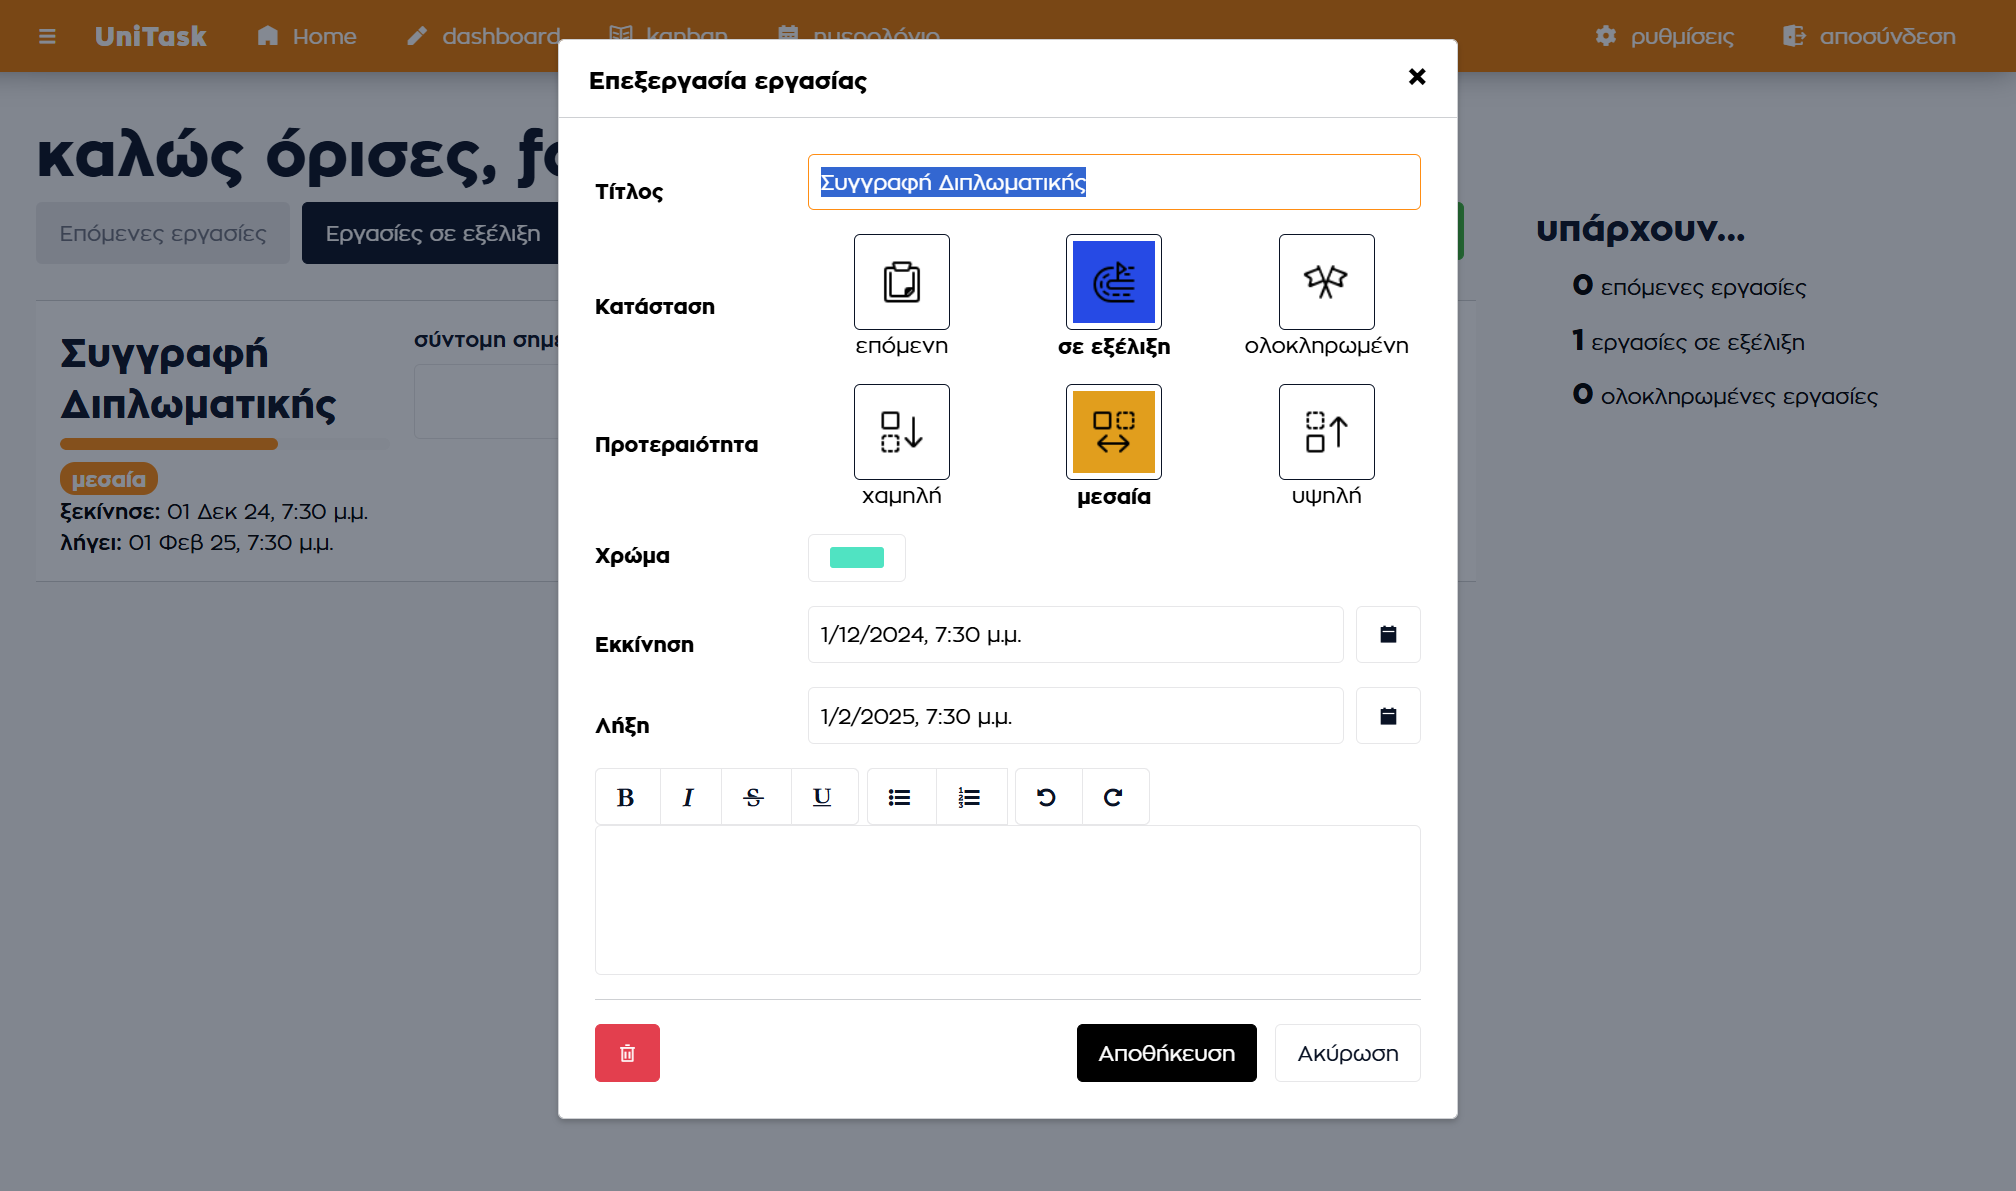
\includegraphics[width=\textwidth]{UniTask/EditTask}
%            \caption{\centering Επεξεργασία εργασίας}
%            \label{fig:unitask_EditTask}
%        \end{figure}
%
%        Πατώντας στο εικονίδιο επεξεργασίας, εμφανίζεται το popout παράθυρο του σχήματος \ref{fig:unitask_EditTask} όπου μπορούν να επεξεργαστούν τα στοιχεία της εργασίας μαζί με το πλαίσιο σύντομης σημείωσης. Το ίδιο παράθυρο περιλαμβάνει και το κουμπί διαγραφής της εργασίας.
%
%        \begin{figure}[h!] \noindent \centering
%            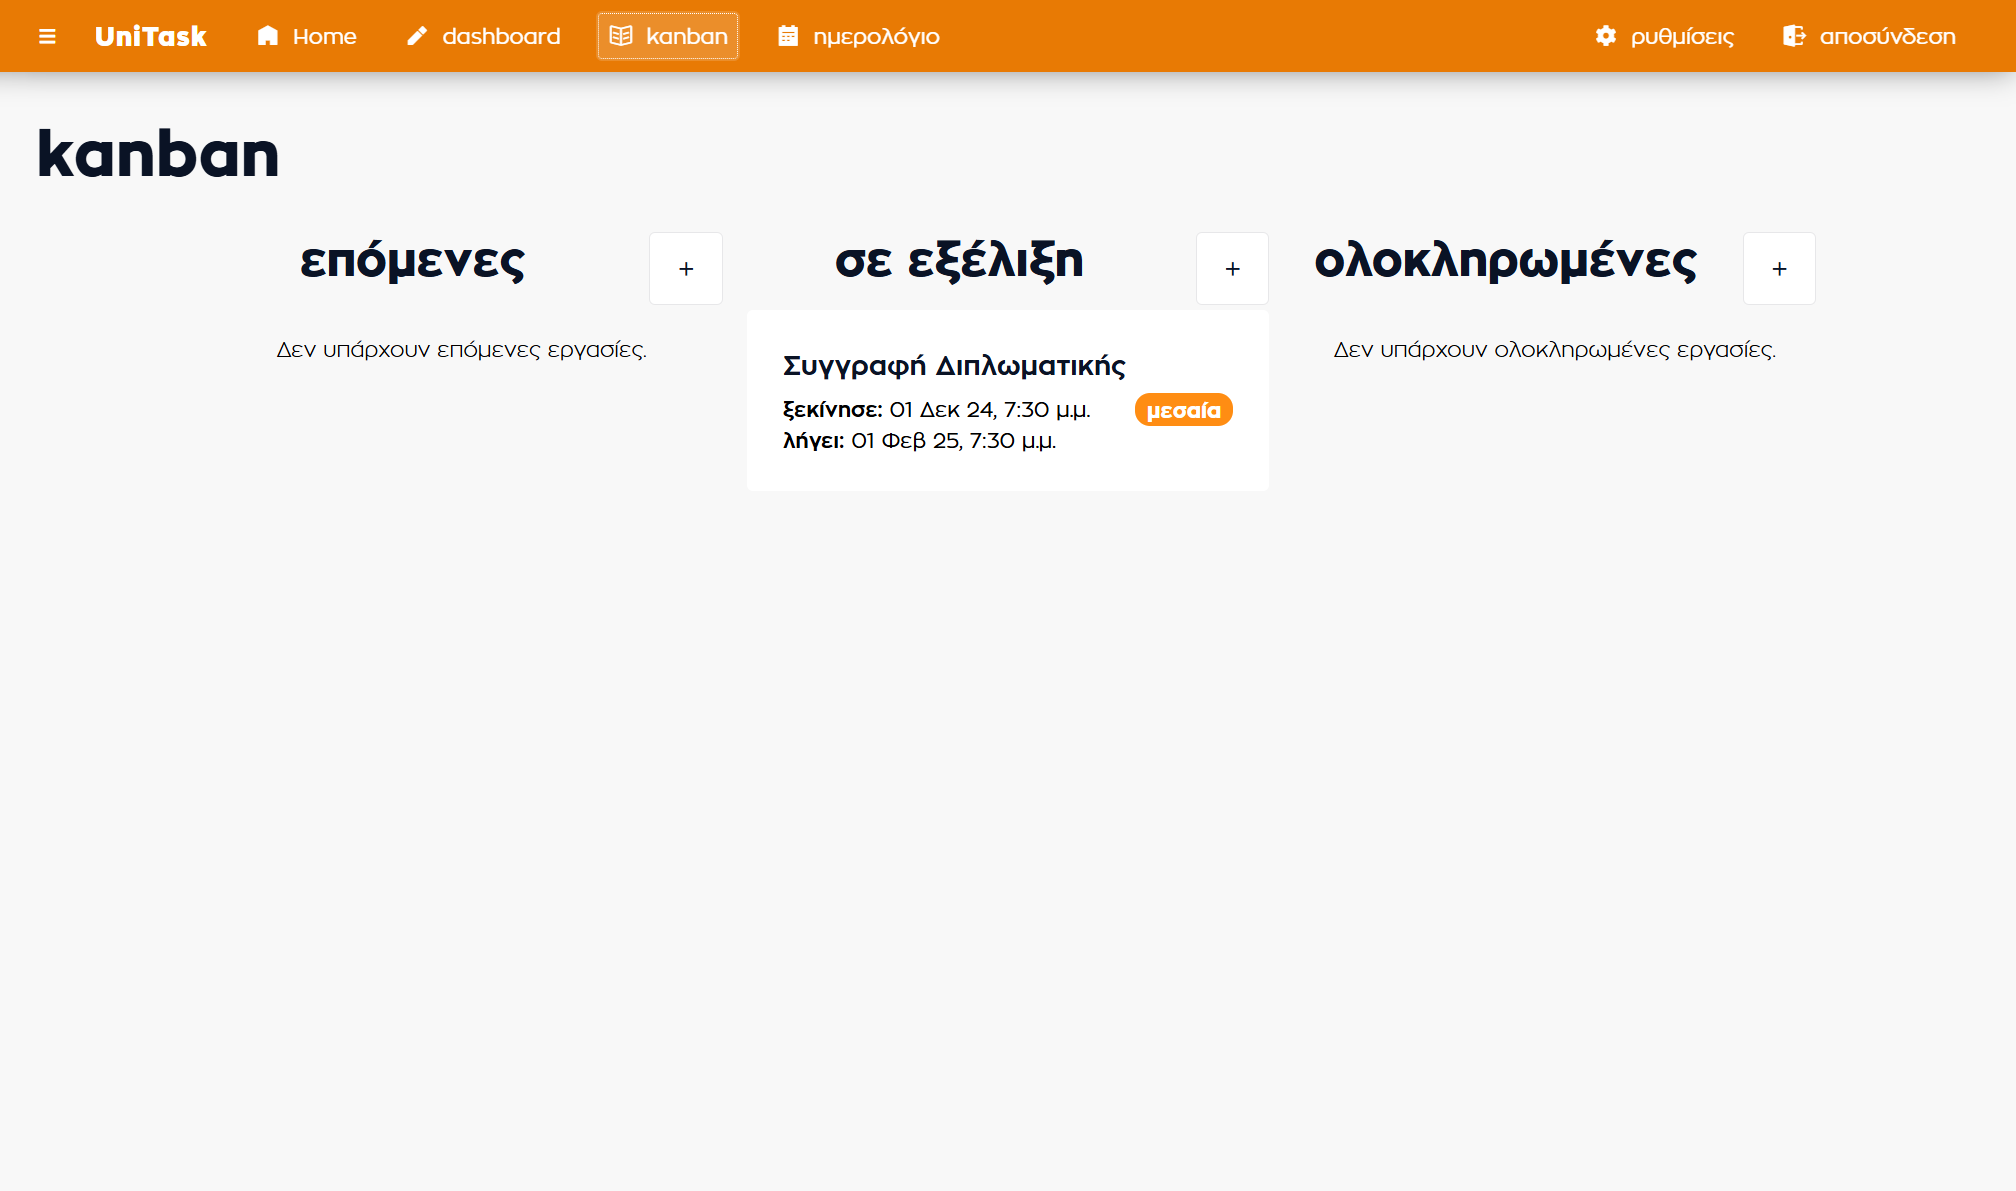
\includegraphics[trim={0 10cm 0 0}, clip, width=\textwidth]{UniTask/Kanban_WithTask}
%            \caption{\centering Σελίδα Kanban}
%            \label{fig:unitask_Kanban_WithTask}
%        \end{figure}
%
%        Η σελίδα {\ZonaSB Kanban} του σχήματος \ref{fig:unitask_Kanban_WithTask} εμφανίζει μια διαφορετική παρουσίαση στις εργασίες με τον τρόπο που έχει εξηγηθεί στην ενότητα \ref{subsec:Kanban}. Στον πίνακα Kanban οι εργασίες χωρίζονται σε τρεις κατηγορίες: τις εργασίες που έχουν ολοκληρωθεί, τις εργασίες που βρίσκονται σε εξέλιξη και τις εργασίες που έχουν σκοπό να πραγματοποιηθούν στο μέλλον. Κάθε στήλη περιλαμβάνει ένα κουμπί δημιουργίας νέας εργασίας που αυτόματα καθορίζει και την κατηγορία της.
%
%        Οι εργασίες εμφανίζονται σε κάρτες με τον τίτλο της εργασίας, την προτεραιότητα της, την ημερομηνία έναρξης και λήξης της, ενώ πατώντας πάνω στην κάρτα μιας εργασίας, εμφανίζεται το popout παράθυρο επεξεργασίας της εργασίας του σχήματος \ref{fig:unitask_EditTask}.
%
%        Στη σελίδα {\ZonaSB ημερολόγιο} (σχήμα \ref{fig:unitask_Calendar_WithTask}) εμφανίζεται ένα ημερολόγιο με τις εργασίες του χρήστη. Οι εργασίες εμφανίζονται στο ημερολόγιο με το χρώμα που έχει οριστεί στην επιλογή του χρήστη κατά τη δημιουργία της εργασίας, υπάρχουν προβολές ανά ημέρα, εβδομάδα ή μήνα ενώ εμφανίζεται και ένα σύντομο παράρτημα στα δεξιά με την λίστα των εργασιών.
%
%        \begin{figure}[h!] \noindent \centering
%            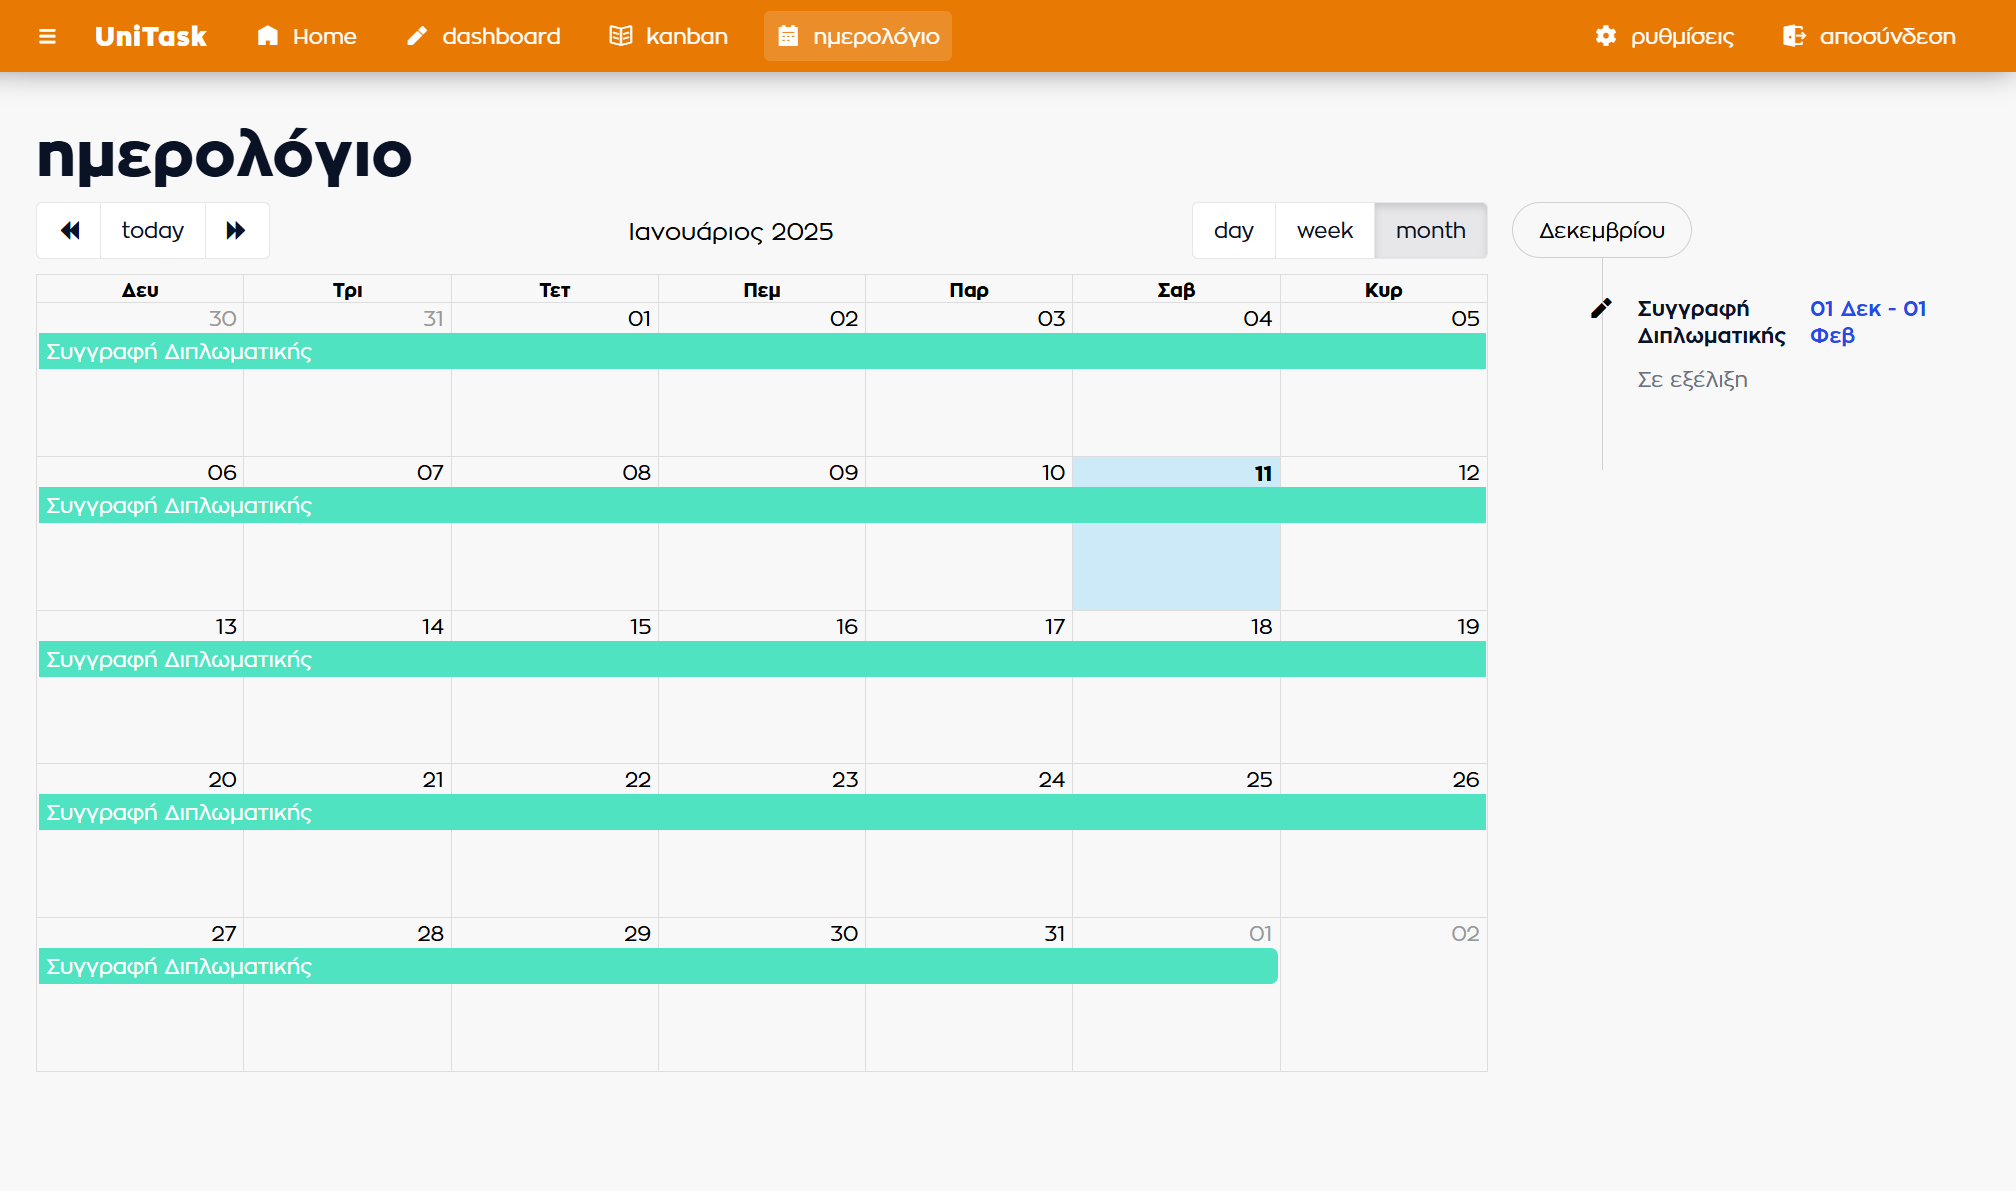
\includegraphics[width=\textwidth]{UniTask/Calendar_WithTask}
%            \caption{\centering Σελίδα Calendar}
%            \label{fig:unitask_Calendar_WithTask}
%        \end{figure}
%
%        Τέλος, στη σελίδα {\ZonaSB ρυθμίσεις} (σχήμα \ref{fig:unitask_Settings}) μπορούμε με ένα κουμπί να διαγράψουμε όλες τις εργασίες μας, ή να επιλέξουμε τη λειτουργία γρήγορης διαγραφής εργασιών. Αυτή η λειτουργία εισάγει ένα κουμπί διαγραφής στις κάρτες εργασιών στο dashboard, επιτρέποντας την άμεση διαγραφή των εργασιών που θέλουμε χωρίς να χρειάζεται να μεταβούμε στη σελίδα επεξεργασίας κάθε εργασίας (σχήμα \ref{fig:unitask_Dashboard_Kanban_Calendar_WithTasks}.1). Τέλος, παρέχεται η δυνατότητα αρχικοποίησης των εργασιών. Στην αρχικοποίηση διαγράφονται οι υπάρχουσες εργασίες του χρήστη και δημιουργούνται κάποιες προκαθορισμένες οι οποίες λειτουργούν ως ένα demo (σχήμα \ref{fig:unitask_Dashboard_Kanban_Calendar_WithTasks}).
%
%        \begin{figure}[h!] \noindent \centering
%            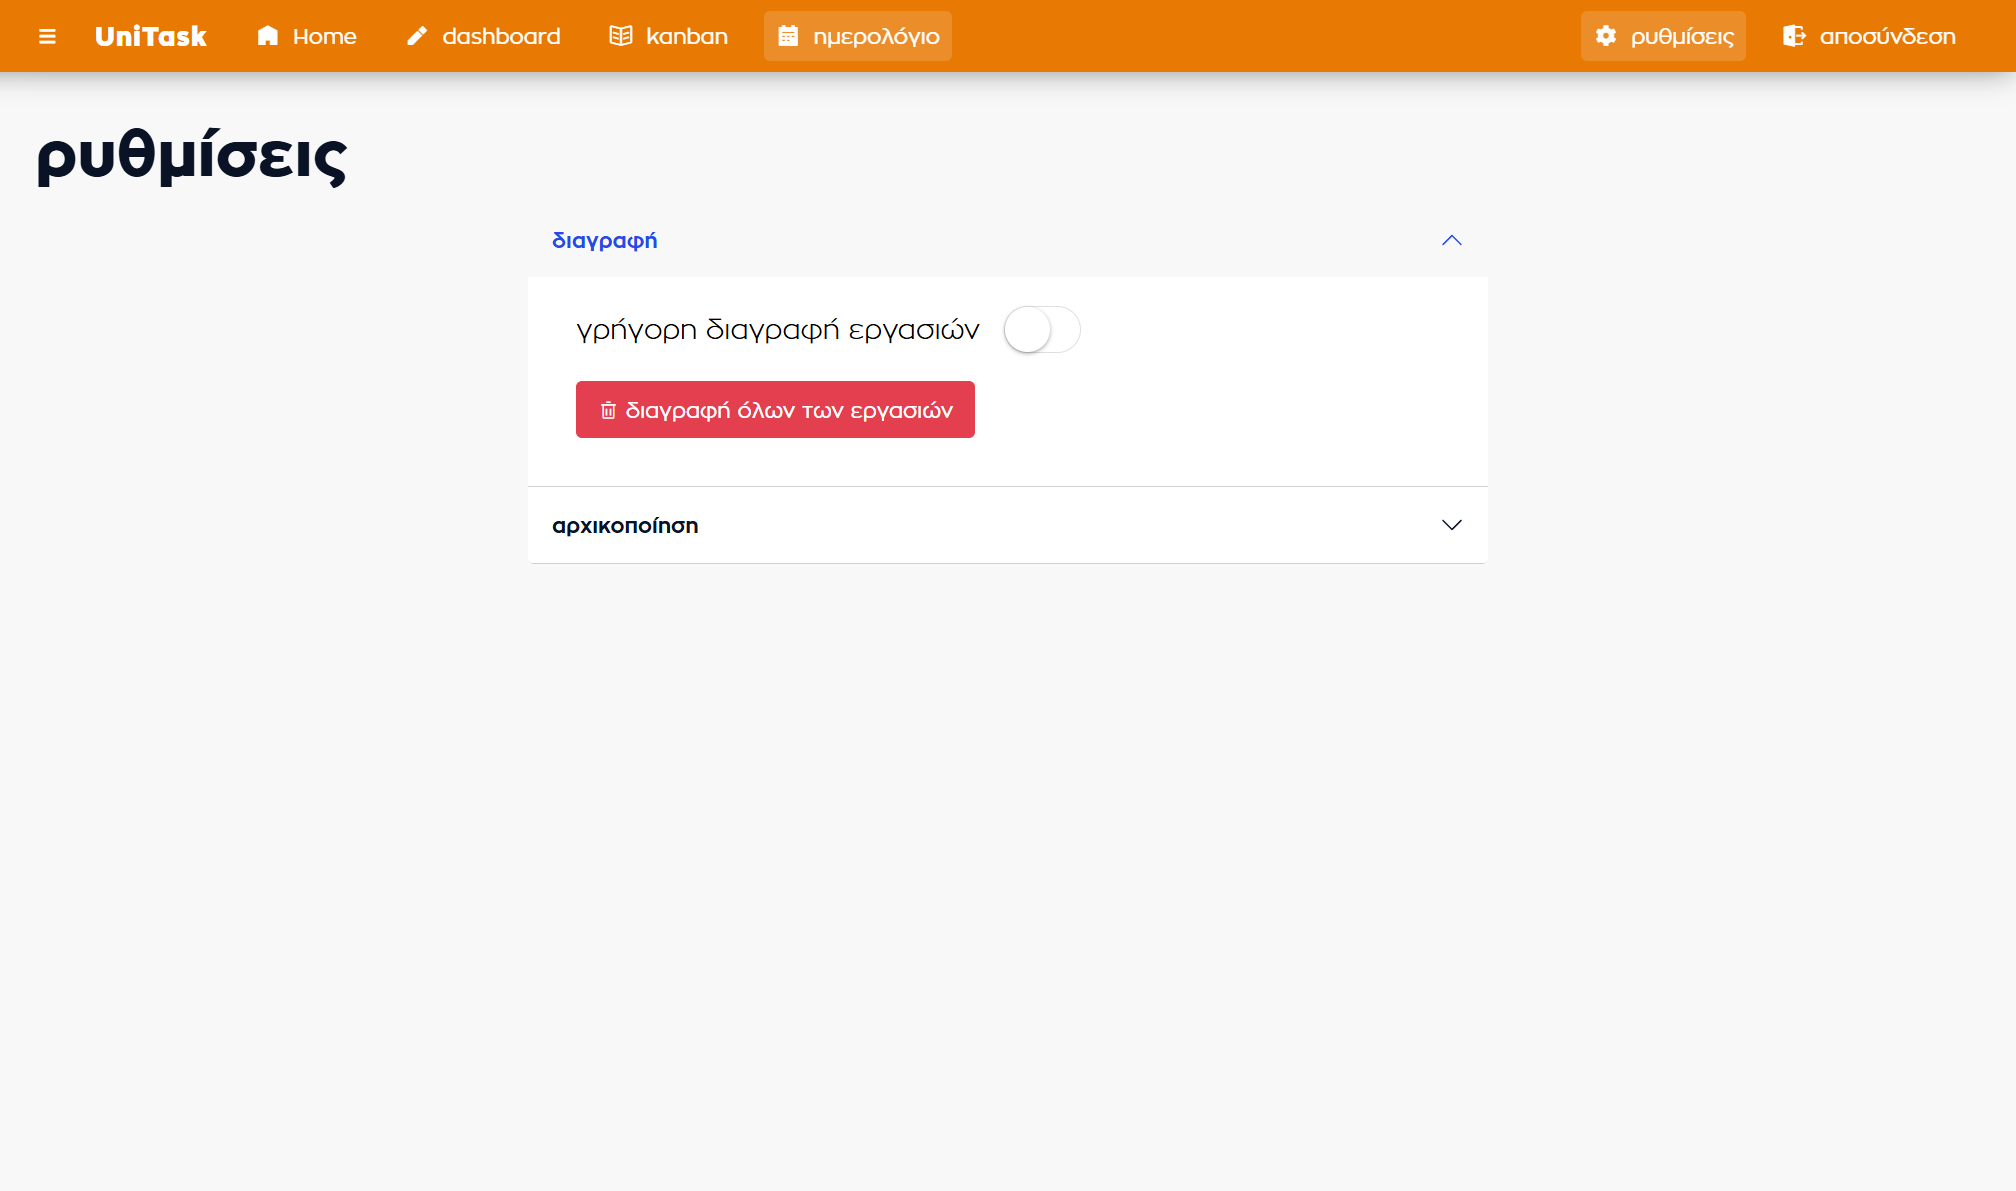
\includegraphics[trim={0 20cm 0 0}, clip, width=\textwidth]{UniTask/Settings_1}
%            
\includegraphics[width=\textwidth]{UniTask/Settings_2}
%            \caption{\centering Σελίδα ρυθμίσεων}
%            \label{fig:unitask_Settings}
%        \end{figure}
%
%        Σε κάθε ρύθμιση εμφανίζονται επιβεβαιωτικά popout μηνύματα προκειμένου να αποφευχθούν ακούσιες διαγραφές εργασιών (σχήμα \ref{fig:unitask_InitializationPopUp}).
%
%        \begin{figure}[h!] \noindent \centering
%            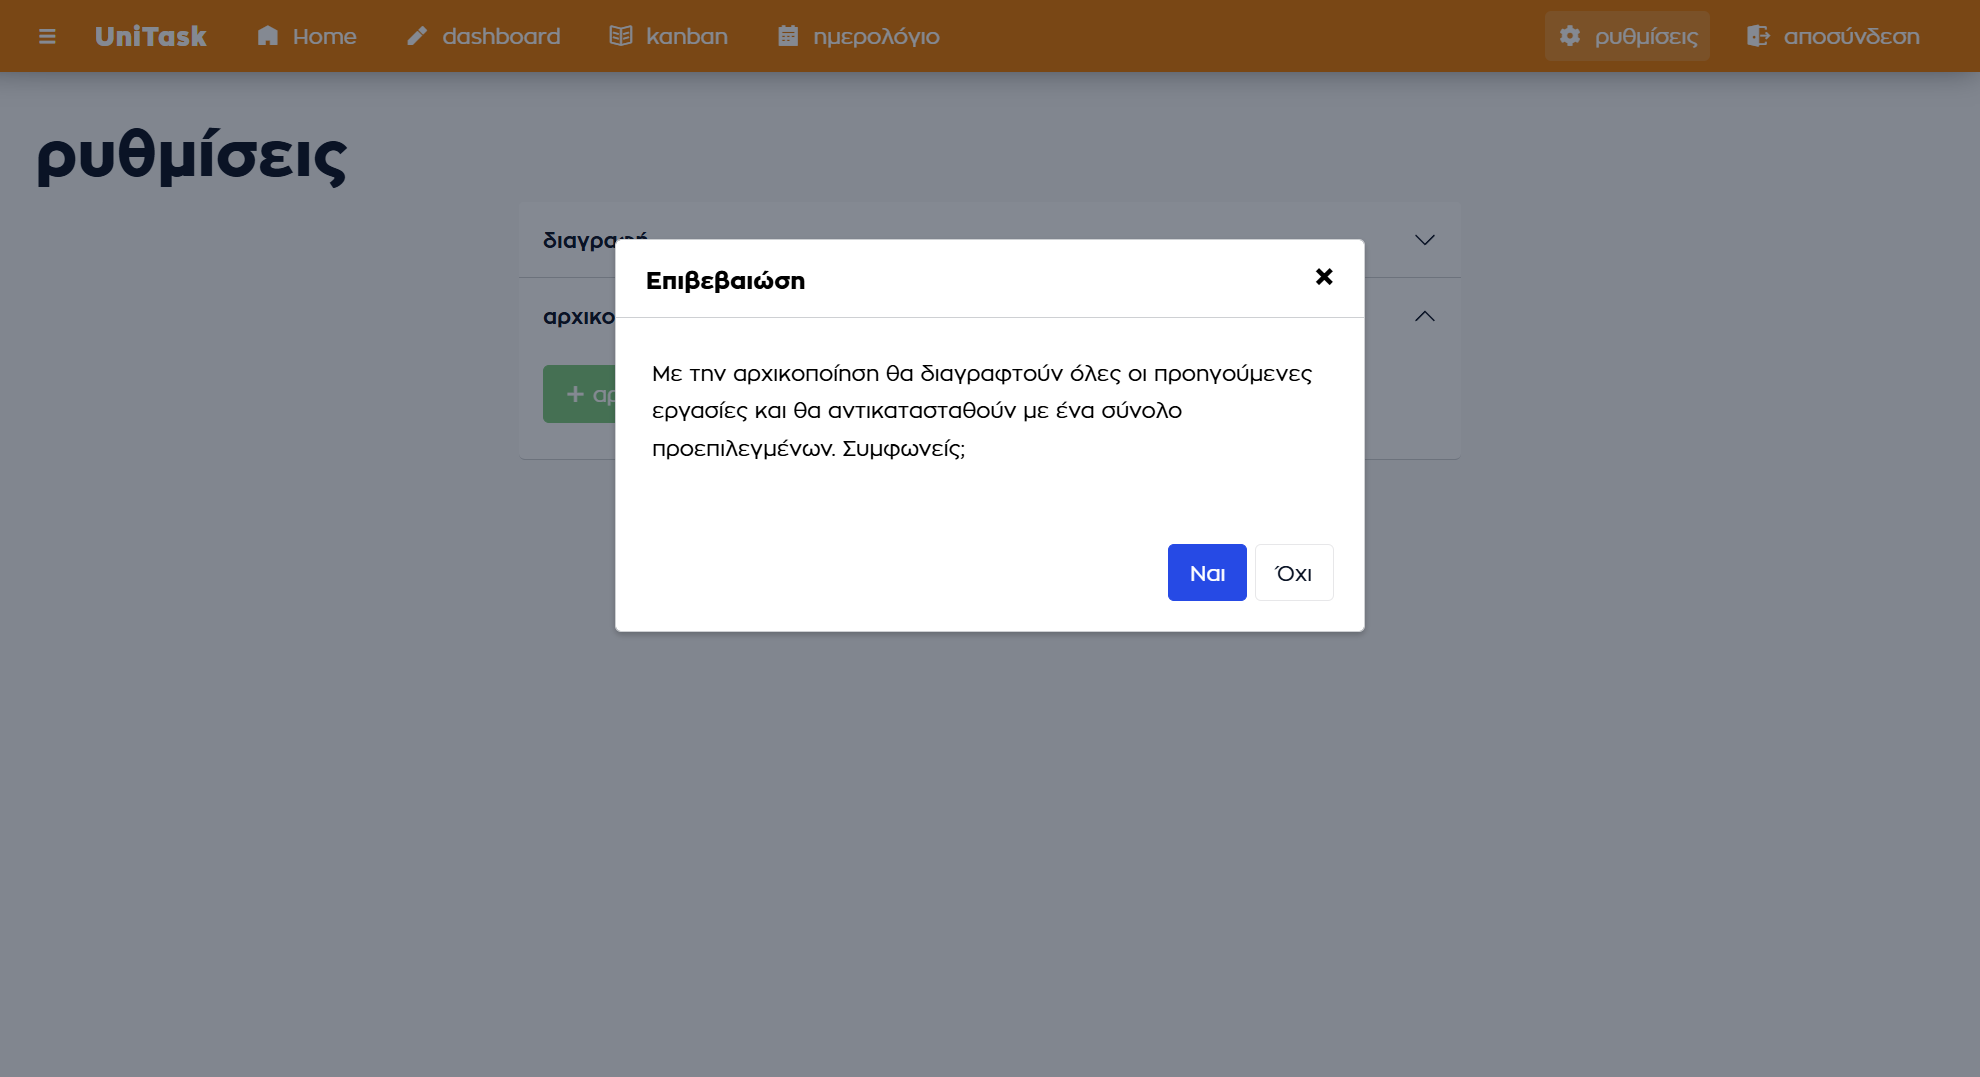
\includegraphics[trim={0 10cm 0 0}, clip, width=\textwidth]{UniTask/InitializationPopUp}
%            \caption{\centering Σελίδα ρυθμίσεων}
%            \label{fig:unitask_InitializationPopUp}
%        \end{figure}
%
%        \begin{figure}[p!] \noindent \centering
%            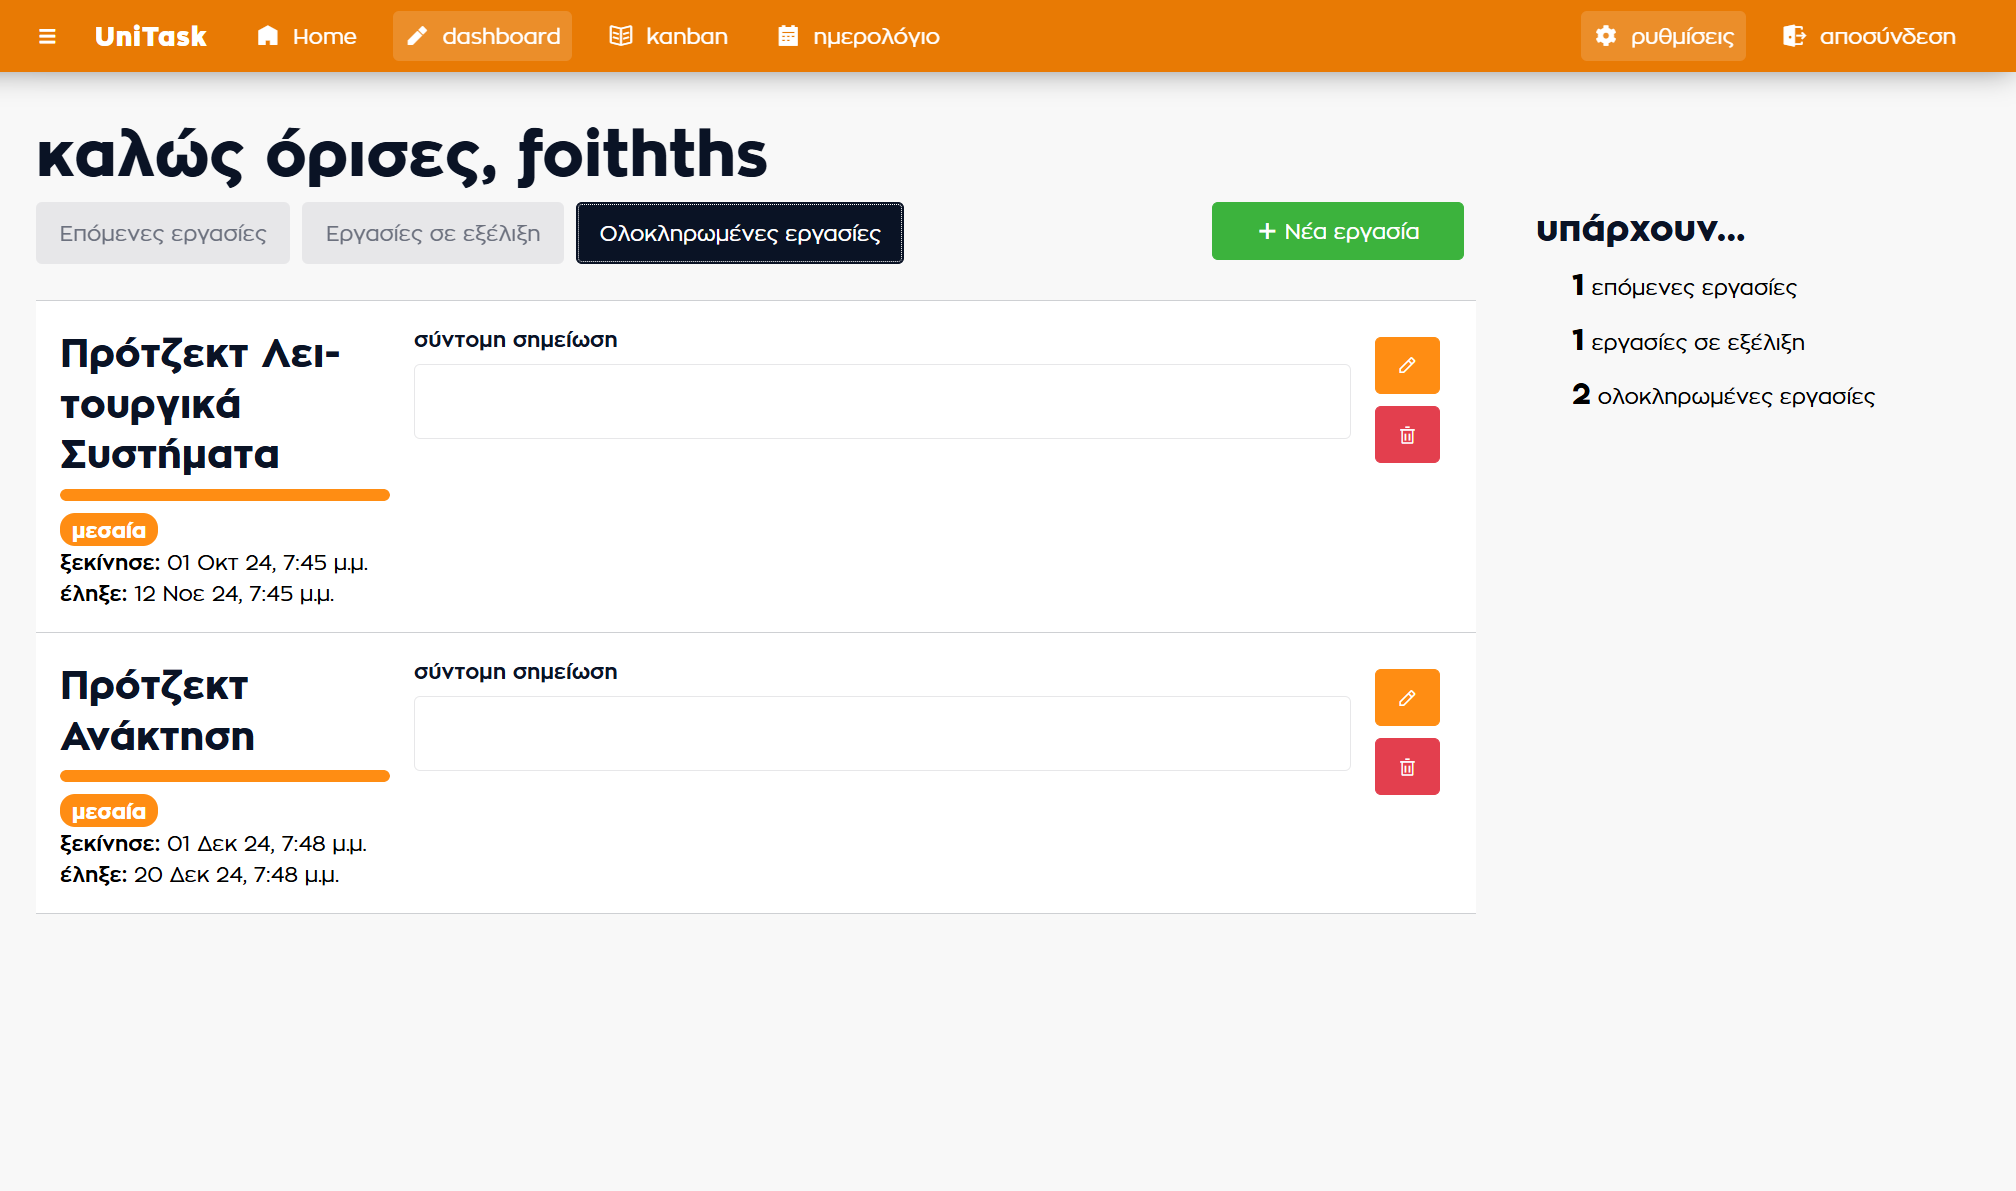
\includegraphics[trim={0 5cm 0 0}, clip, width=\textwidth]{UniTask/TaskDashboard_QuickDelete}
%            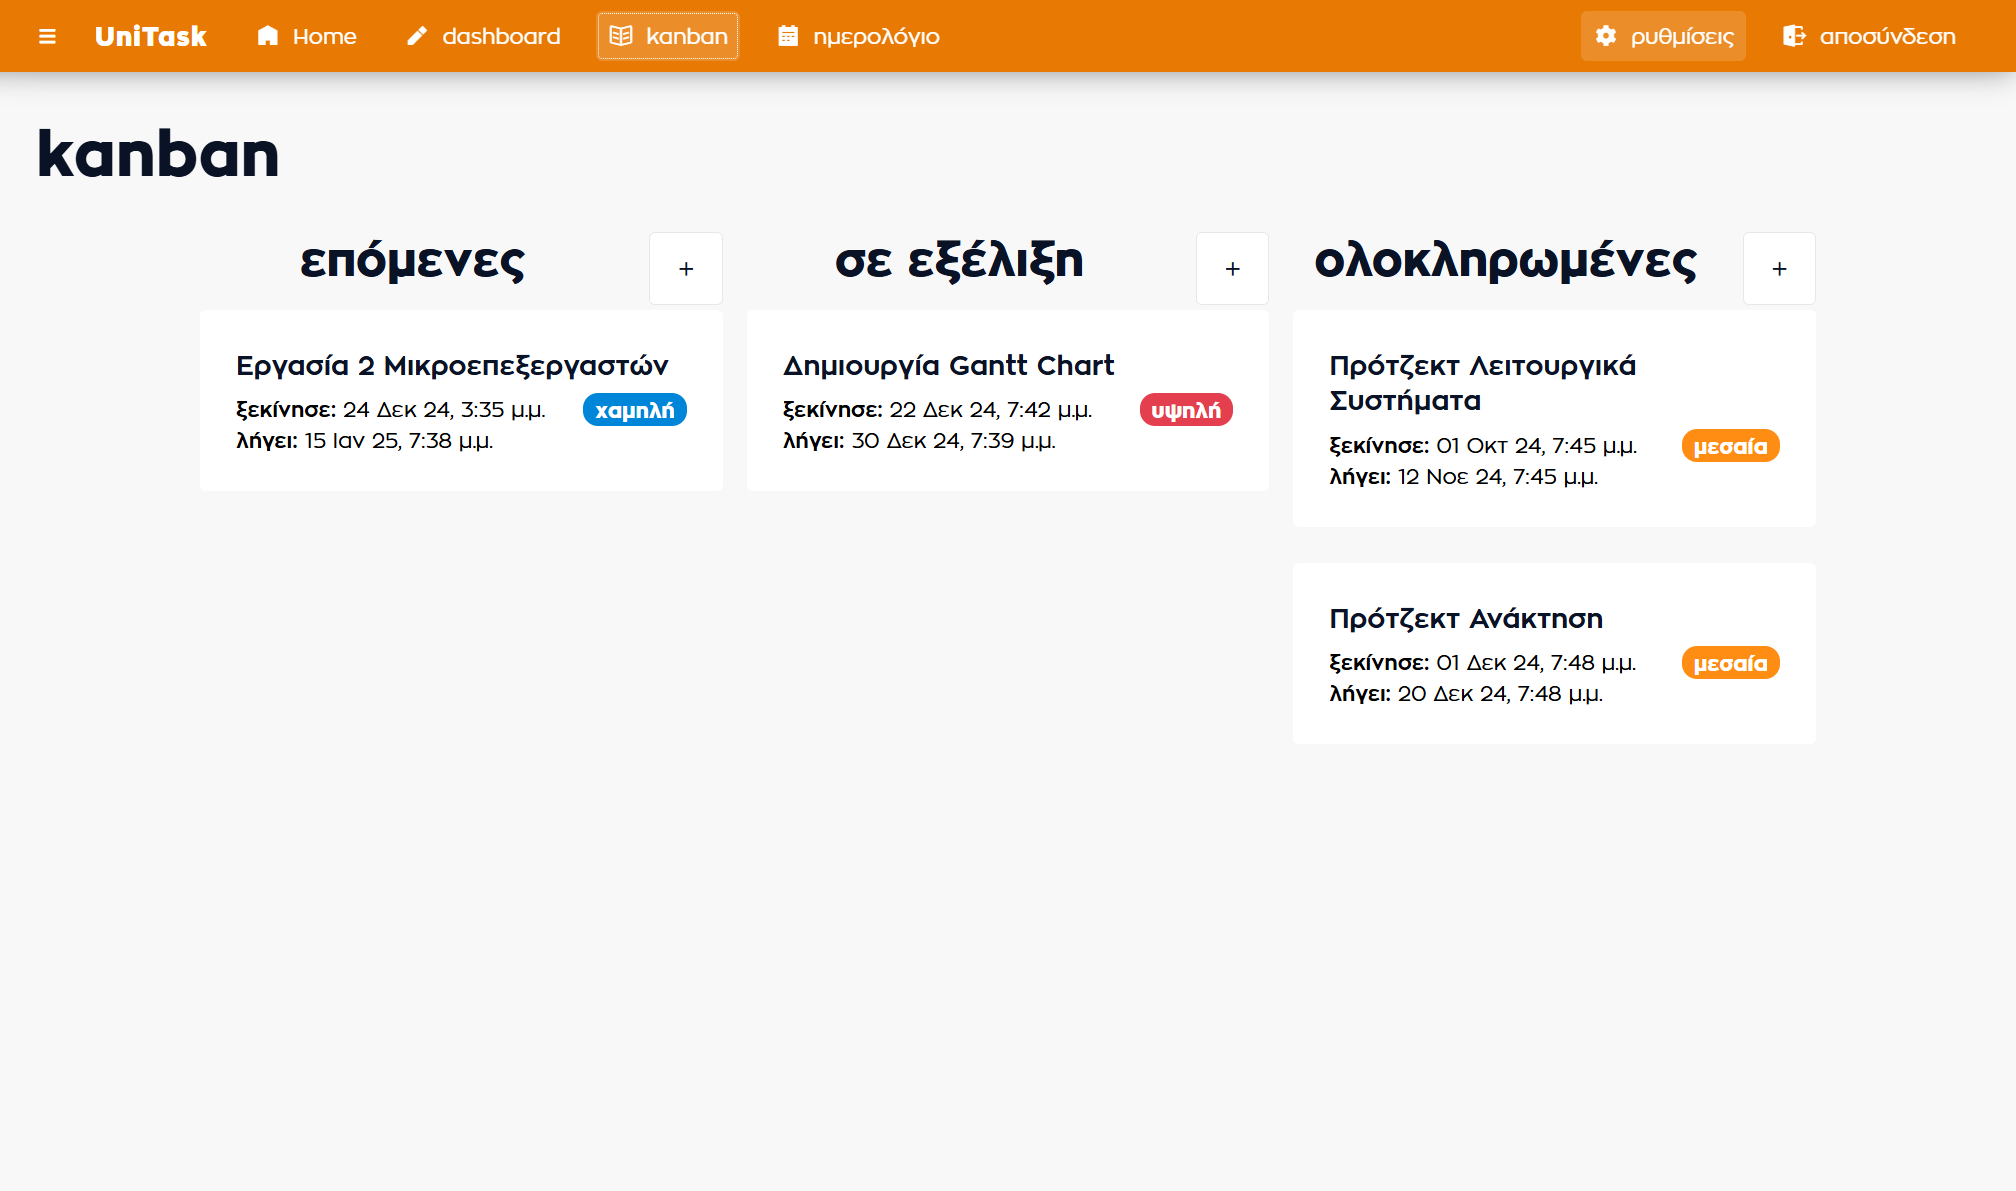
\includegraphics[trim={0 10cm 0 0}, clip, width=\textwidth]{UniTask/Kanban_WithTasks}
%            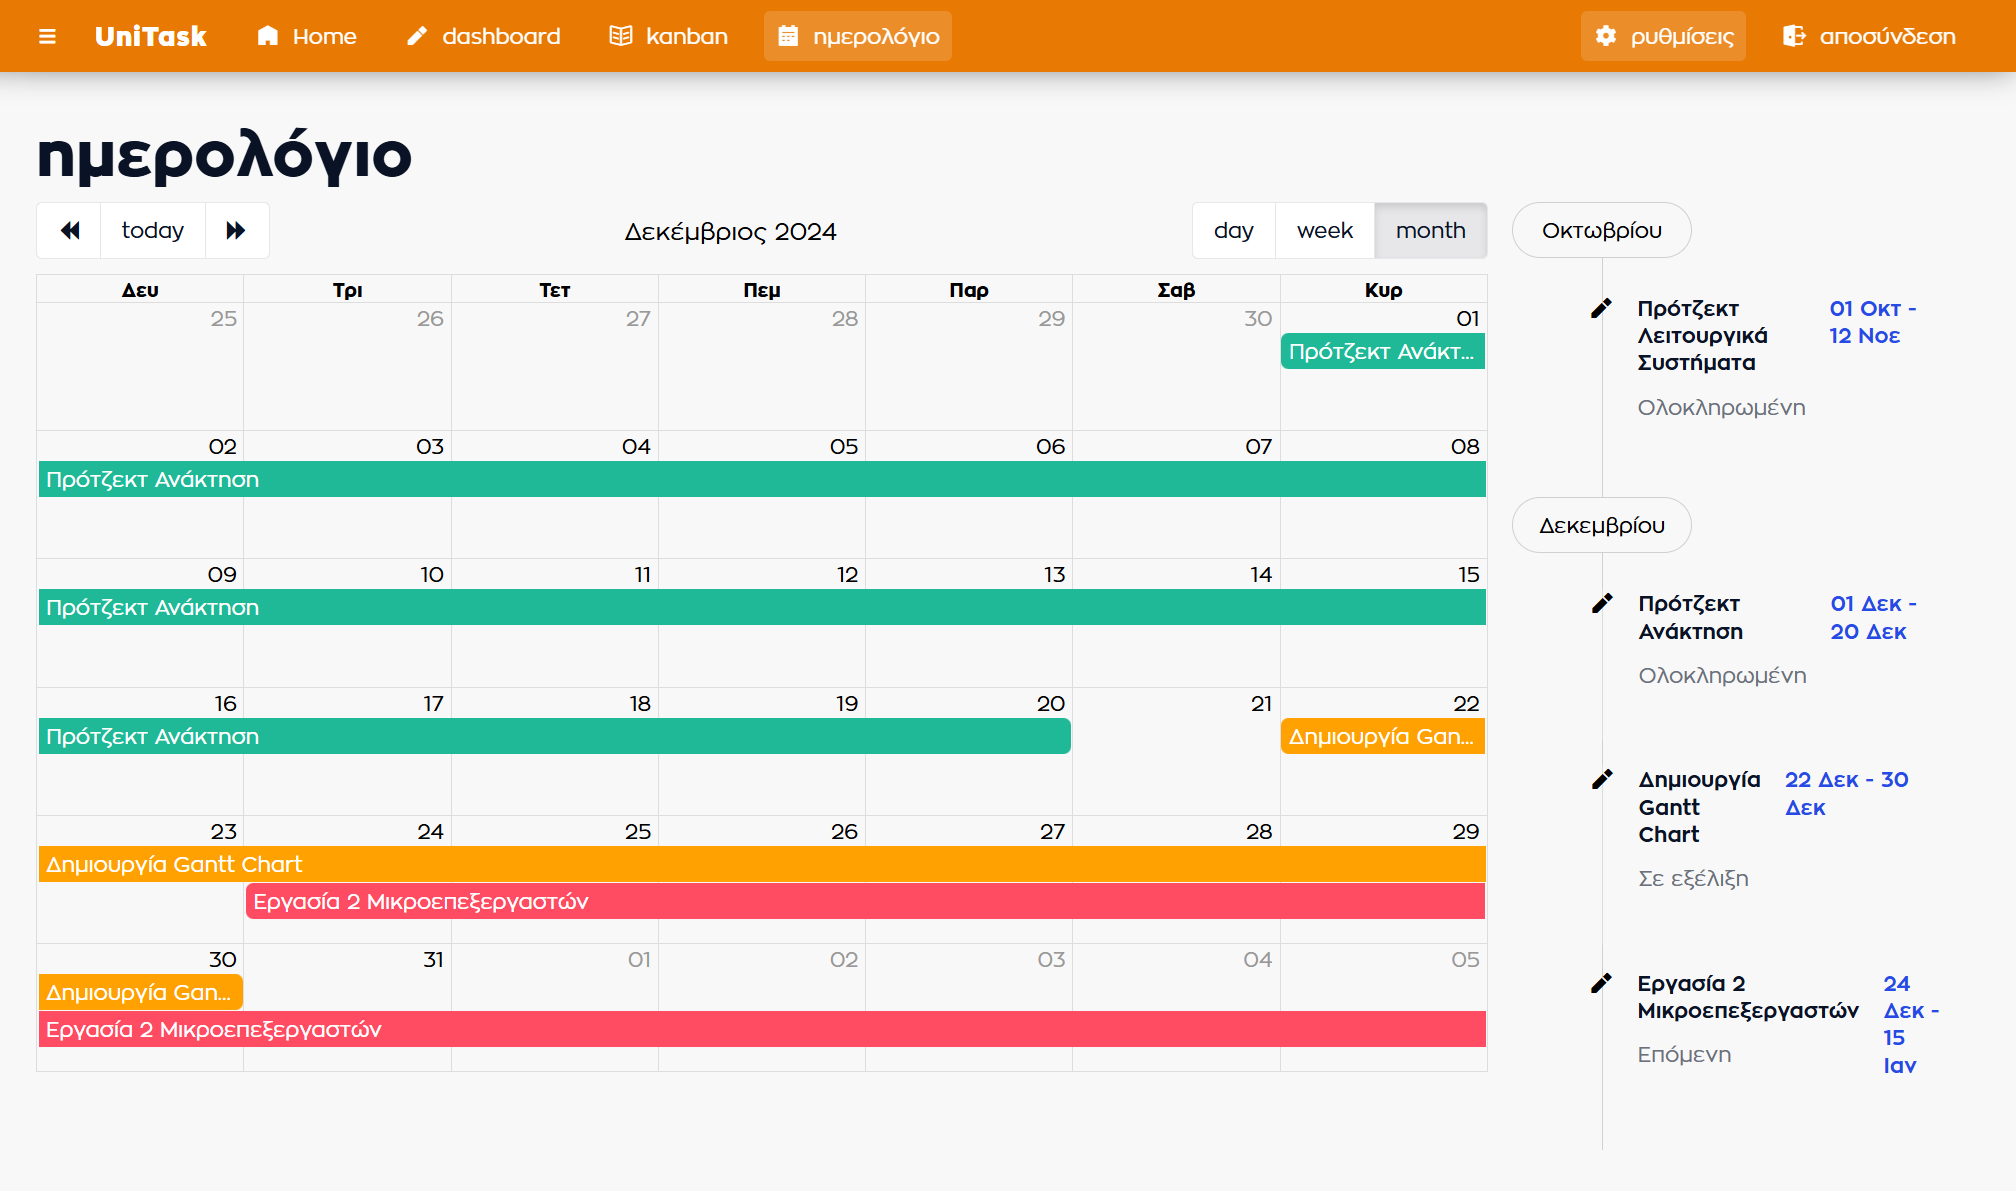
\includegraphics[width=\textwidth]{UniTask/Calendar_WithTasks}
%            \caption{\centering Οι σελίδες Dashboard, Kanban και Calendar μετά την αρχικοποίηση των εργασιών. Στο Dashboard φαίνεται η λειτουργία γρήγορης διαγραφής εργασιών.}
%            \label{fig:unitask_Dashboard_Kanban_Calendar_WithTasks}
%        \end{figure}

    \section{Δομή της εφαρμογής} \label{sec:unitask_mendix}
        Πέρα από τα προκατασκευασμένα modules του Mendix, η λειτουργικότητα της εφαρμογής έχει οργανωθεί σε τρία modules, το \texttt{Administrator}, το \texttt{TaskManager} και το \texttt{UniTask}.

        \subsection{Module \texttt{Administrator}}
            Το \texttt{Administrator} περιλαμβάνει τη λειτουργικότητα που αφορά τη διαχείριση των χρηστών της εφαρμογής.
            \subsubsection{Domain model του Administrator}

            \subsubsection{Σελίδες του Administrator}
                Στο \texttt{Administrator} περιλαμβάνονται οι εξής σελίδες:
                \paragraph{\texttt{Account\_Overview}}
                    \begin{center}
                        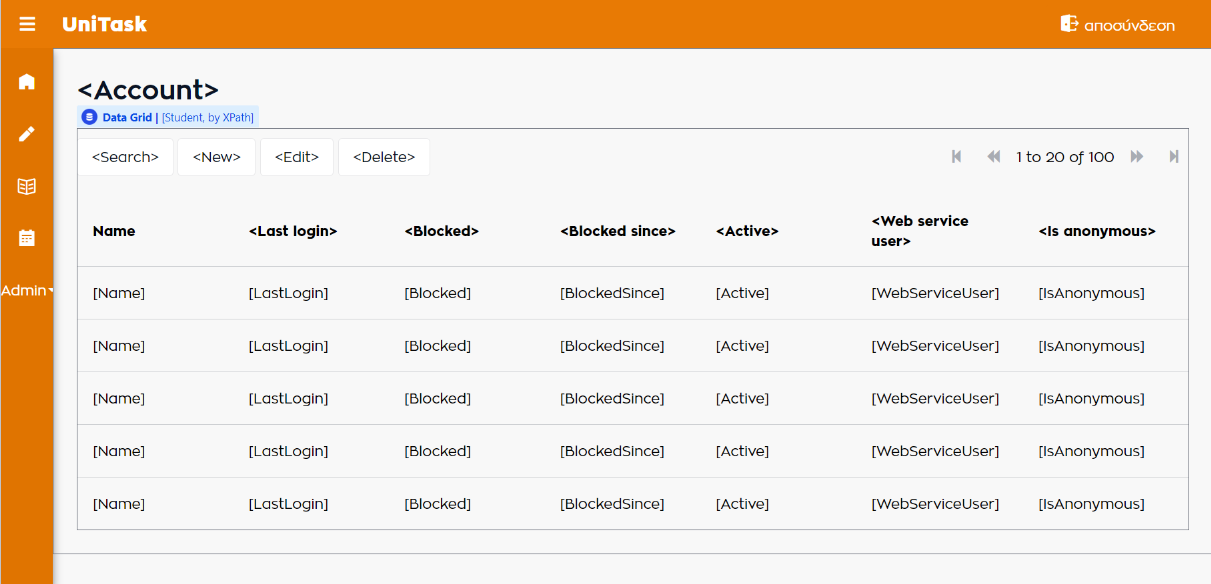
\includegraphics[width=0.9\textwidth]{UniTask_Mendix/Account_Overview}
                    \end{center}

                    Η σελίδα χρησιμοποιείται για τη διαχείριση των χρηστών της εφαρμογής από την πλευρά των διαχειριστών.

                    Χρησιμοποιείται το \texttt{UniTask\_SideBar} layout του \texttt{UniTaskDesignSystem} module. Το κύριο μέρος της σελίδας αποτελείται από ένα Data Grid με Data source την οντότητα \texttt{Student} και με στήλες τις ιδιότητες \texttt{Name}, \texttt{Last login}, \texttt{Blocked}, \texttt{Blocked since}, \texttt{Active}, \texttt{Web service user} και \texttt{Is anonymous}.

                \paragraph{\texttt{Account\_New}}
                    \begin{center}
                        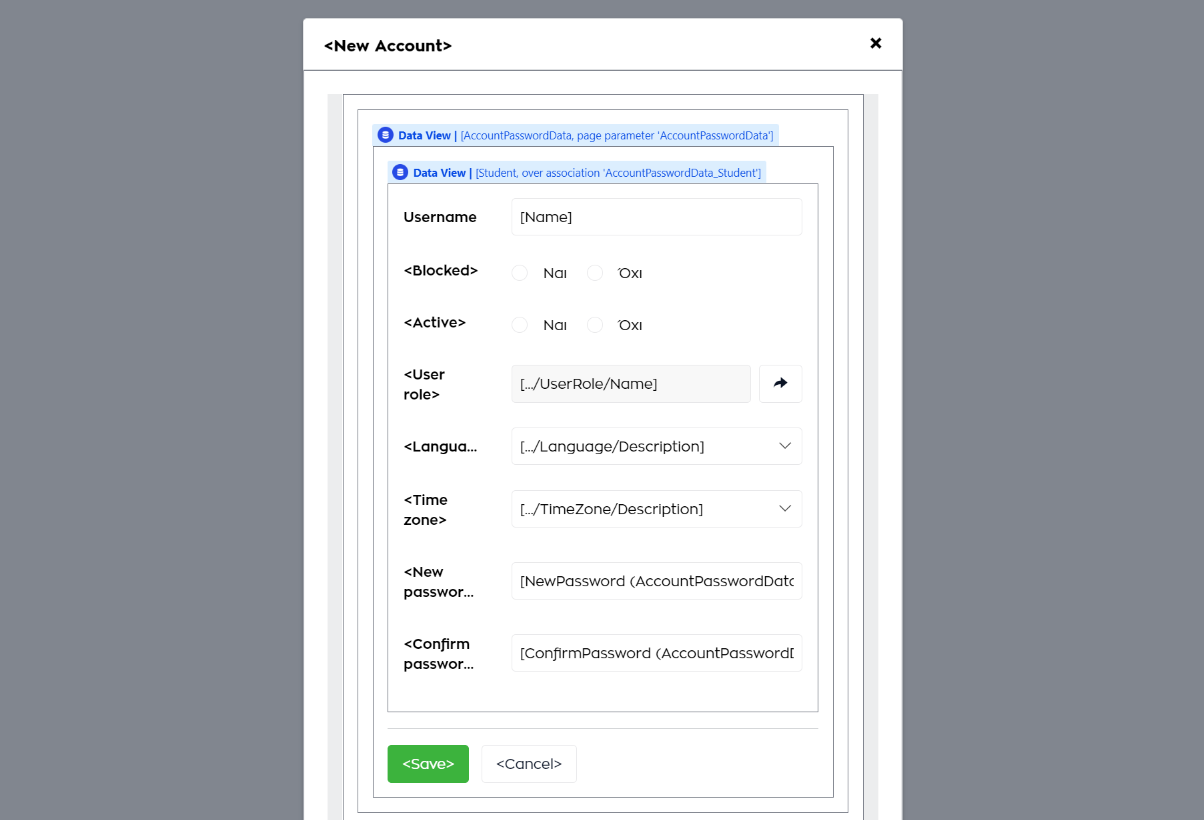
\includegraphics[width=0.9\textwidth]{UniTask_Mendix/Account_New}
                    \end{center}

                    Η σελίδα χρησιμοποιείται για τη δημιουργία νέων χρηστών της εφαρμογής.

                    Χρησιμοποιείται το \texttt{PopupLayout} layout του \texttt{Atlas\_Core} module. Η σελίδα περιλαμβάνει δύο Parameters, το \texttt{Student} και \texttt{AccountPasswordData} του module \texttt{Administrator}. Η σελίδα αποτελείται από δύο εμφωλευμένα Data Views, το εξωτερικό έχει ως Data source το \texttt{AccountPasswordData}, ενώ το εσωτερικό έχει ως Data source τη συσχέτιση του \texttt{AccountPasswordData} με το \texttt{Student}. Η χρήση του \texttt{AccountPasswordData} είναι απαραίτητη καθώς η δημιουργία ενός νέου χρήστη χρειάζεται την αποθήκευση του κωδικού πρόσβασής του.

                    Στο εσωτερικό Data View περιλαμβάνει Text Boxes, Radio Buttons και Input \linebreak Reference Set Selectors όπου εισάγονται τιμές για τα \texttt{Username}, \texttt{Blocked}, \texttt{Active}, \texttt{User role}, \texttt{Language}, \texttt{Time zone}, \texttt{New password} και \texttt{Confirm password}. Έχει σημασία να σημειωθεί πως οι ιδιότητες (γνωρίσματα) που αποθηκεύουμε στην πραγματικότητα δεν είναι ιδιότητες του \texttt{Student} αλλά του \texttt{System.User} του οποίου αποτελεί παιδί. Το Input Reference Set Selector χρησιμοποιείται για την επιλογή του \texttt{UserRole}, που αποτελεί διαφορετική σελίδα που θα αναλυθεί στη συνέχεια.

                    Τέλος, περιλαμβάνεται κουμπί για την αποθήκευση, το οποίο καλεί το microflow \texttt{ACT\_Account\_Save} του \texttt{Administrator} για την αποθήκευση των τιμών, και κουμπί για την ακύρωση της διαδικασίας.

                \paragraph{\texttt{Account\_Edit}}
                    \begin{center}
                        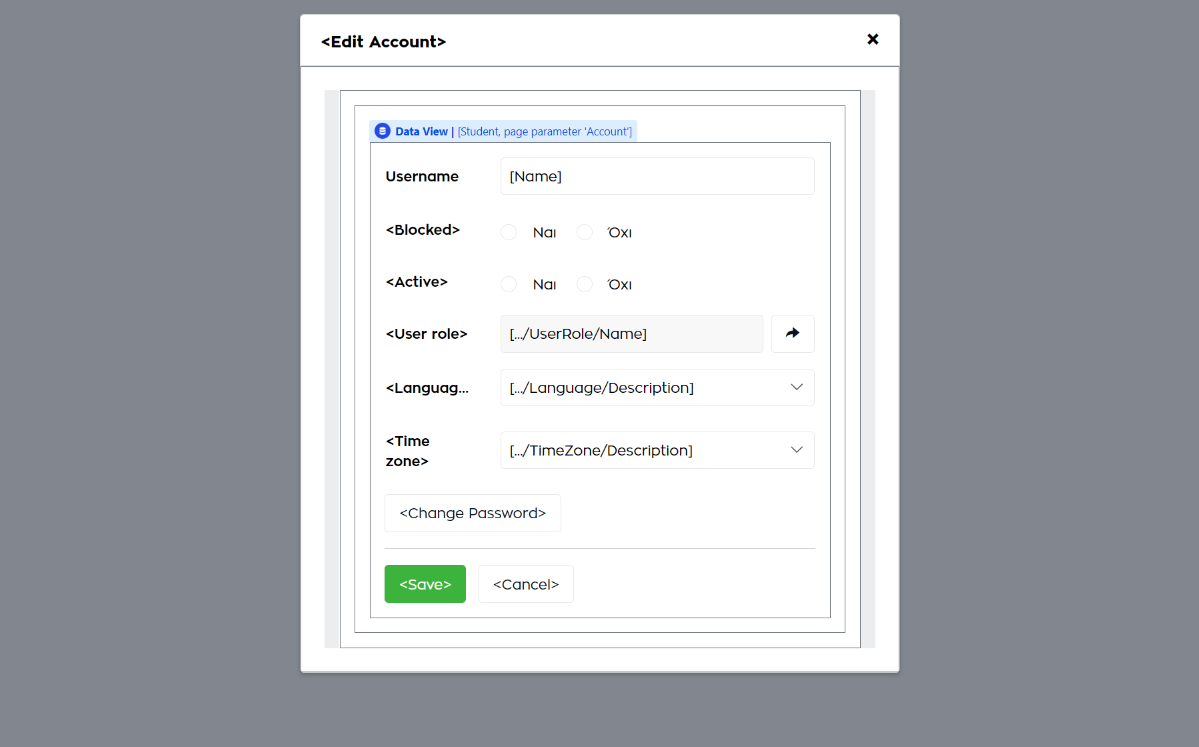
\includegraphics[width=0.9\textwidth]{UniTask_Mendix/Account_Edit}
                    \end{center}

                    Η σελίδα χρησιμοποιείται για την επεξεργασία υπαρχόντων χρηστών της εφαρμογής.

                    Χρησιμοποιείται το \texttt{PopupLayout}. Η σελίδα περιλαμβάνει το Parameter \texttt{Student}. Η σελίδα αποτελείται από ένα Data View με Data source το \texttt{Student} με παρόμοια Text Boxes και Radio Buttons όπως και το \texttt{Account\_New}. Επίσης, περιλαμβάνεται το κουμπί που καλεί το microflow \texttt{ACT\_Password\_Change} για την αλλαγή κωδικού.

                    Τέλος, περιλαμβάνεται κουμπί για την αποθήκευση και κουμπί για την ακύρωση της διαδικασίας. Τα κουμπιά καλούν προεπιλεγμένες ενέργειες του Mendix.

                \paragraph{\texttt{Change\_Password}}
                    \begin{center}
                        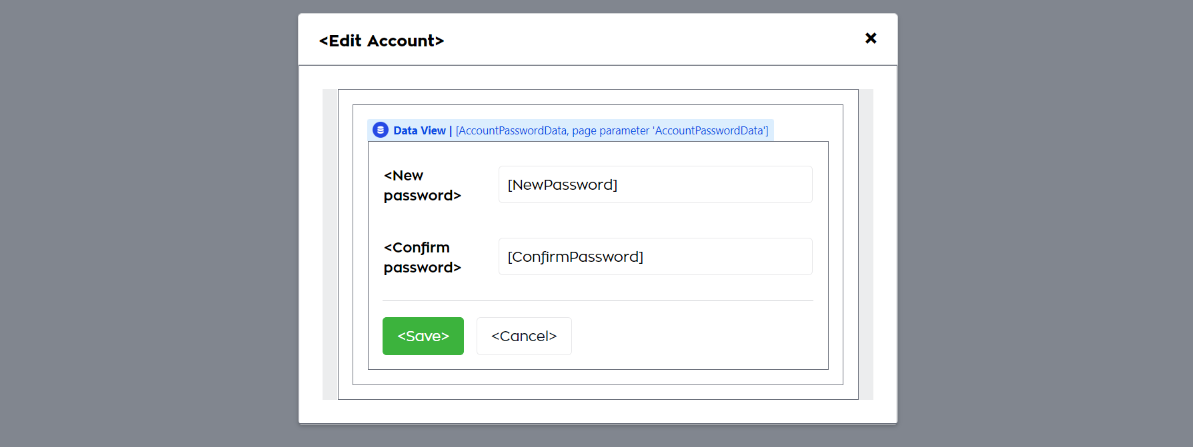
\includegraphics[width=0.9\textwidth]{UniTask_Mendix/Change_Password}
                    \end{center}

                    Η σελίδα χρησιμοποιείται για την αλλαγή του κωδικού πρόσβασης υπάρχοντος χρήστη.

                    Χρησιμοποιείται το \texttt{PopupLayout}. Η σελίδα περιλαμβάνει το Parameter \linebreak \texttt{AccountPasswordData}, ένα Data View με Data source το \texttt{Student} με τα απαραίτητα Text Boxes για την αλλαγή των τιμών. Τέλος, περιλαμβάνεται κουμπί για την αποθήκευση που καλεί το microflow \texttt{ChangePassword} του \texttt{Administrator} και κουμπί για την ακύρωση της διαδικασίας.

                \paragraph{\texttt{UserRole\_Select}}
                    \begin{center}
                        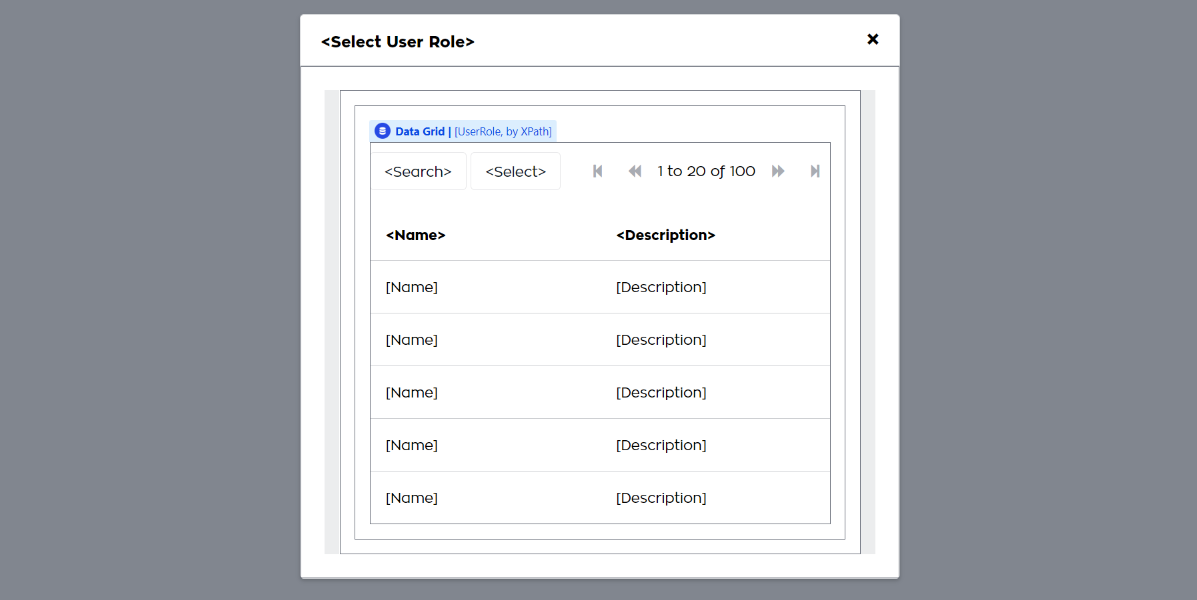
\includegraphics[width=0.9\textwidth]{UniTask_Mendix/UserRole_Select}
                    \end{center}

                    Η σελίδα χρησιμοποιείται για την επιλογή του ρόλου του χρήστη κατά τη δημιουργία νέου χρήστη.

                    Χρησιμοποιείται το \texttt{PopupLayout}.